\chapter{Dinámica neuronal experimental del C. elegans}\label{cap:resultado_critico}
\graphicspath{{figs/capitulo_resultado_critico/}}

\chapterquote{dynamical systems with extended spatial
	degrees of freedom naturally evolve into self-organized critical structures of states which
	are barely stable. The combination of dynamical minimal stability and spatial scaling
	leads to a power law for temporal fluctuations}{Bak}

Este apartado presenta los resultados de los experimentos realizados con datos experimentales del nematodo C. elegans. El objetivo central de este análisis es examinar si el sistema nervioso de este organismo exhibe características de criticidad neuronal. Para lograrlo, se recopilaron datos de actividad neuronal en gusanos inmovilizados proporcionados por investigaciones previas y se aplicaron diversas métricas. Estos experimentos proporcionarán una comprensión más profunda acerca de si el C. elegans muestra propiedades típicas de la criticidad neuronal a nivel microscópico.

Este apartado se centra en la exposición de los datos experimentales recopilados, los métodos empleados en su análisis y, en última instancia, los resultados obtenidos. Exploraremos en detalle las métricas de criticidad aplicadas y cómo estas han revelado patrones y propiedades específicas en la actividad neuronal. También examinaremos las implicaciones de estos resultados en el contexto de nuestra hipótesis principal y su posible relevancia en los campos de la neurociencia y la investigación computacional.

A lo largo de este apartado, se evaluará la coherencia de los hallazgos con la teoría de la criticidad neuronal y cómo estos resultados contribuyen a una comprensión más completa de la dinámica neuronal en el C. elegans. Además, se considerarán las posibles limitaciones y alcances de estos resultados experimentales.


%Las cuatro características que acabamos de describir se observan comúnmente en sistemas complejos que experimentan una transición de fase orden-desorden [1, 10, 13]. Este escenario fue explorado en [58] definiendo un parámetro de control y un parámetro de orden a partir de los datos
%
%Para representar el grado de orden (es decir, el parámetro de orden), se calculó el tamaño del grupo más grande (normalizado por el número de sitios activos) en todo el cerebro y se representó en función del número de puntos activos (es decir, el parámetro de control). Esto se hizo para todos los pasos de tiempo y se representó en la Figura 3.7e (círculos pequeños). Como parámetro de control, se utilizó el nivel global de actividad como en otros modelos bien estudiados de transiciones orden-desorden (el ejemplo más claro es la percolación [59]).
%
%
%El mismo razonamiento lleva a la conjetura [1, 6, 7] de que la complejidad de la dinámica cerebral es solo otra firma de un proceso crítico subyacente. Debido a que el mayor número de estados metaestables existe en el punto cercano a la transición, el cerebro puede acceder al mayor repertorio de comportamientos de manera flexible. Esa visión afirmó que las propiedades más fundamentales del cerebro solo son posibles manteniéndose cerca de esa inestabilidad crítica, independientemente de cómo se alcance o mantenga dicho estado. En las siguientes secciones, se analiza la evidencia empírica reciente que apoya esta hipótesis.
%La presencia de escalado y correlaciones que abarcan el tamaño del sistema suelen ser indicios de fenómenos críticos. Si bien, en principio, es relativamente sencillo identificar estas firmas, en el caso de datos finitos y la ausencia de una teoría formal, como es el caso del cerebro, cualquier indicio inicial de criticidad debe verificarse con muchos artefactos conocidos. En los próximos párrafos, discutimos los esfuerzos más relevantes para identificar estas firmas en datos cerebrales a gran escala.
%
%a aplicación de este nuevo método permitió, por primera vez, definir un marco teórico en términos de un parámetro de orden y control derivado de los datos de fMRI, donde el régimen dinámico puede interpretarse como uno correspondiente a un sistema cercano al punto crítico de una transición de fase de segundo orden. El análisis demostró que el cerebro en reposo pasa la mayor parte del tiempo cerca del punto crítico de dicha transición y exhibe avalanchas de actividad regidas por las mismas propiedades dinámicas y estadísticas descritas anteriormente para los eventos neuronales a escalas más pequeñas.
%
%Esto se explora aquí compilando las estadísticas y la dinámica de los grupos de puntos tanto en el espacio como en el tiempo. Los grupos son grupos de vóxeles contiguos con señales por encima del umbral en un momento dado, identificados por un algoritmo de escaneo en cada volumen de fMRI. La Figura 3.7a muestra ejemplos de grupos (en este caso no consecutivos en el tiempo) representados con diferentes colores. Por lo general (Figura 3.7b, arriba), el número de grupos en un momento dado solo varía un orden de magnitud alrededor de la media (50). Por el contrario, el tamaño del grupo activo más grande fluctúa ampliamente, abarcando más de cuatro órdenes de magnitud.


%\chapterquote{...Why should it take an infinite amount of logic to figure out what a tiny piece of space/time is going to do? So I have often made the hypothesis that ultimately physics will not require a mathematical  statement, that in the end the machinery will be revealed, and the laws will turn out to be simple, like the chequer board with all its apparent complexities }{Richard P. Feynman}

%
%Los resultados presentados en esta Carta muestran que se pueden predecir aspectos muy relevantes de la dinámica cerebral a partir de la estructura, siempre que la dinámica subyacente sea crítica. Para guiar nuestra comparación con los resultados experimentales disponibles, elegimos concentrarnos en hallazgos sólidos sobre la dinámica cerebral. Específicamente, preguntamos cómo la dinámica cerebral espontánea a gran escala se organiza en los relativamente pocos patrones espaciotemporales revelados experimentalmente en los últimos años [4]. Esto es importante porque una amplia gama de experimentos que utilizan imágenes de resonancia magnética funcional (fMRI) ha enfatizado que estos grupos espaciales de actividad coherente, denominados redes de estado de reposo (RSN) [5], están específicamente asociados con sistemas neuronales responsables de sensorial, cognitiva, y funciones conductuales
%
%
%El cerebro animal está compuesto por miles de millones de neuronas, que interactúan entre sí a través de miles de sinapsis por neurona. El resultado de tal interacción es la aparición de patrones espaciotemporales complejos de actividad neuronal que respaldan la percepción, la acción y el comportamiento. Una propuesta reciente considera al cerebro como una red de neuronas preparadas cerca de una transición dinámica [1–4], un punto de vista que está respaldado por resultados experimentales obtenidos de animales tanto in vitro [5] como in vivo [6], así como de estudios completos. experimentos humanos de neuroimagen cerebral [7-9].
%
%
%
%% Homeostatic plasticity and emergence of functional networks in a whole-brain model at criticality
%Estas ideas han sido particularmente investigadas en los últimos quince años en neurociencia y la hipótesis de que el cerebro está cerca de un estado crítico (en mecánica estadística sensu) está ganando consenso en la comunidad neurocientífica14,17,23–25. En los sistemas cerebrales, el concepto de criticidad está respaldado principalmente por los siguientes dos hallazgos experimentales: (i) el descubrimiento de avalanchas neuronales libres de escala19, como se describe mediante distribuciones de ley de potencia para el tamaño y la duración de los estallidos espontáneos de actividad en la corteza; (ii) la presencia de correlaciones temporales de largo alcance en las fluctuaciones de amplitud de las oscilaciones neuronales26,27. Otros estudios informaron sobre la universalidad de los exponentes de la ley de potencia encontrados originalmente en 19 entre diferentes especies, por ejemplo, rata28; primates no humanos29,30 y humanos mediante diversas técnicas, como MEG31–33; EEG34 y fMRI15,35. También desde un punto de vista teórico, muchos modelos de cerebro completo describen al máximo las actividades neuronales reales cuando se encuentran en un punto crítico15,19,35–38.
%
%
%
% La hipótesis emergente es que los sistemas vivos, o partes de ellos, como el cerebro, se acercan espontáneamente a una transición de fase crítica (estrictamente hablando, las transiciones de fase existen solo para sistemas con un número infinito de grados de libertad, que en el mejor de los casos son una buena aproximación de sistemas grandes, pero finitos, como un cerebro)16,17, lo que les confiere las características emergentes de los sistemas críticos como la falta de escalas espaciales y temporales y la alta capacidad de respuesta a las perturbaciones externas. Estas características se traducirían en la capacidad del cerebro, a través de una actividad de gran escala espacial y temporal, para reaccionar rápidamente ante estímulos externos generando un comportamiento global coordinado18, para maximizar la transmisión de información19,20, la sensibilidad a los estímulos sensoriales 21 y el almacenamiento de información22.
%
%
%
%
%Desde un punto de vista teórico, la física estadística ha contribuido decisivamente a resaltar la ventaja potencial que puede tener un cerebro en un estado crítico y también proporciona una descripción cuantitativa de las actividades cerebrales a través de modelos mesoscópicos minimalistas14,15. Los sistemas que constan de muchos componentes microscópicos (p. ej., neuronas) pueden exhibir tipos bastante diversos de comportamiento colectivo macroscópico con diferentes niveles de organización interna (p. ej., actividad cerebral). Además, ligeros cambios en los estímulos externos (p. ej., auditivos, visuales, etc.) o en la fuerza de las propias interacciones pueden inducir cambios estructurales drásticos, es decir, transiciones de fase. Por lo tanto, es tentador plantear la hipótesis de que los estados biológicos podrían ser manifestaciones de fases colectivas similares y que los cambios entre ellos podrían corresponder a transiciones de fase.
%
%
%
%La hipótesis del cerebro crítico establece que las redes neuronales biológicas, debido a su arquitectura estructural y funcional, trabajan cerca de las transiciones de fase para una respuesta óptima a las entradas internas y externas. Por lo tanto, la criticidad proporciona funciones y capacidades de comportamiento óptimas. Este capitulo pureba  esta hipótesis en la dinamica neuronal de C. elegans reales examinando la influencia de la lesión cerebral (ictus) en la criticidad de la dinámica neuronal estimada a nivel de sujetos individuales utilizando modelos de cerebro completo.
%
%
%Recientemente se ha encontrado evidencia de dinámica crítica tanto en experimentos como en modelos de dinámica cerebral a gran escala.
%
%Encontramos que la variación de los parámetros topológicos puede dar lugar a un comportamiento invariante de escala que pertenece a la clase de universalidad de percolación de campo medio o que tiene exponentes críticos no universales.
%
%El estudio de la actividad funcional cerebral ha revelado la existencia de fluctuaciones correlacionadas e invariancia de escala similares a las observadas en los fenómenos críticos. Tal evidencia provocó la conjetura de que la organización a gran escala del cerebro emerge en la criticidad [1-3].
%
%
%
%
%
%El documento está organizado de la siguiente manera. en la seg. II se describe el modelo, así como los métodos de simulación y escalado de tamaño finito utilizados. Los resultados se presentan en la Sec. tercero Discutimos la relevancia de los principales hallazgos en la Sec. IV.
%


%\section{Introducción}



%Traducción al español:
%
%En estas notas, discutimos la idea propuesta hace dos décadas por Bak [1] de que el cerebro en funcionamiento se mantiene en un régimen intermedio (crítico) caracterizado por correlaciones de ley de potencia. Una dinámica cerebral altamente correlacionada produce estados sincronizados sin valor conductual, mientras que una dinámica débilmente correlacionada impide el flujo de información. Entre estos estados, las características dinámicas únicas del estado crítico dotan al cerebro de propiedades que son fundamentales para el comportamiento adaptativo. Esta simple propuesta está ahora respaldada por un amplio conjunto de pruebas empíricas a diferentes escalas, que demuestran que la dinámica espaciotemporal del cerebro exhibe las firmas clave de la dinámica crítica, previamente reconocidas en otros sistemas complejos.
%
%
%Los circuitos neuronales muestran complejos patrones de actividad temporal espontáneos y evocados por estímulos. Como los transitorios de calcio dentro de las neuronas individuales reflejan uno o más eventos de potenciales de acción, la coincidencia temporal de los transitorios de calcio entre las neuronas ofrece una oportunidad para caracterizar la estructura de la red.  Una característica destacada de los sistemas dinámicos interconectados es su capacidad para sincronizarse (Acebrón et al., 2005). In vivo, la sincronización desempeña un papel más general al unir grupos de ensamblajes neuronales distribuidos en unidades funcionales para que estos ensamblajes puedan transferir información más fácilmente (Melloni et al., 2007; Uhlhaas et al., 2008; Uhlhaas y Singer, 2006; Womelsdorf et al., 2007). Para identificar grupos de neuronas con un patrón de actividad similar y cuantificar su sincronía	

%
%Realizamos simulaciones para varios valores del parámetro de control T que los resultados previos [16] indican que produce dinámicas subcríticas (para valores muy altos de T), supercríticas (para valores muy bajos de T) o críticas. Para acumular suficientes estadísticas, ejecutamos 20 simulaciones numéricas (que duran 105 pasos de tiempo, descartando los 5000 pasos de tiempo iniciales). Para cada simulación construimos una red con los mismos parámetros promedio  k y pi  (es decir, son realizaciones estocásticas). Para imitar situaciones experimentalmente relevantes, registramos la dinámica de las neuronas dentro de una ventana cuadrada de neuronas W × W (con W <= L), vea la Fig. 1-a.
%
%Si el sistema presenta un punto crítico similar a la percolación, se espera que tanto s como S 2 exhiban un máximo (dependiente del tamaño) para un cierto valor pseudocrítico del parámetro de control (el umbral T en el presente caso)
%
%
%Para caracterizar la transición entre estos regímenes se definió un parámetro de orden considerando los tamaños de los clusters activos. Los clústeres son grupos de nodos activados simultáneamente y vinculados entre sí a través de un w distinto de cero. En cada paso de tiempo se calcularon los tamaños del grupo más grande (S1) y el segundo grupo más grande (S2). 
%
%
%n un valor intermedio, un punto crítico [Tc en el panel (c) de la Fig. 1] puede identificarse por el pico en el tamaño del segundo grupo más grande, como se hace generalmente en percolación [16], así como recientemente en IRMf humana experimentos [10]. El tamaño finito del conectoma disponible hace que la demostración habitual de criticidad en el límite termodinámico no sea práctica; por lo tanto, en su lugar, se proporciona una gama de indicadores alternativos (ver también el Material Suplementario [17])
%
%Como ya se mencionó, la distribución de tamaños de conglomerados de actividad puede ser informativa de los diferentes regímenes dinámicos del modelo. Calculamos tales medidas como una función del umbral T
%
%
%
%Como se discutió en el \cref{cap:dinamica_critica} los mecanismos fundamentales que subyacen a la dinámica de la actividad cerebral aún se desconocen en gran medida. La investigación neurocientífica interdisciplinaria, inspirada en la física estadística, ha sugerido que la dinámica neuronal del cerebro de los organismos permanece cerca de un estado crítico, es decir, en la vecindad de una fase crítica de transición entre orden y desorden, o entre actividad oscilatoria asincrónica o sincrónica.  De  hecho, los sistemas neuronales parecen mostrar características  de los sistemas en estado crítico. Estos incluyen i) la invariancia de escala de las avalanchas neurales  reportadas en diversas especies, por ejemplo, ratas \cite{gireesh_neuronal_2008}, primates no humanos \cite{petermann_spontaneous_2009, yu_higher-order_2011}, imágenes de calcio de cerebro completo de pez cebra \cite{ponce-alvarez_whole-brain_2018}  y humanos a través de diferentes técnicas de imagen y señales electrofisiológicas; ii) la presencia de correlaciones espacio-temporales de largo alcance en las fluctuaciones de amplitud de las oscilaciones neuronales, incluida la observación de espectros de potencia $1/ f$ de señales MEG/EEG registradas simultáneamente.  iii)   la distribución del tamaño de los clústeres  en señales BOLD de la conectividad estructural del cerebro humano  \cite{haimovici_brain_2013}. 
%
%Por otra parte  desde mediados de la década de los 90, la intrigante dinámica del cerebro en reposo ha atraído un creciente cuerpo de investigación en neurociencia. Los estudios de neuroimagen han revelado distintas redes funcionales que se activan y desactivan lentamente, lo que apunta a la existencia de una dinámica de red subyacente que emerge espontáneamente durante el reposo, con características espaciales, temporales y espectrales específicas. Si bien la actividad en reposo  se mide comúnmente en humanos, ha sido menos común hacerlo en modelos animales debido a limitaciones técnicas. Sin embargo, se han aplicado técnicas de imagen  en animales, pero generalmente requieren anestesia o fijación de la cabeza. Más recientemente, los avances en la obtención de imágenes de sensores de voltaje o calcio in vivo han sido reconocidos como otro enfoque para evaluar la conectividad funcional en modelos animales despiertos. Se han logrado avances significativos con estas técnicas, que ahora pueden generar imágenes de miles de neuronas y grandes volúmenes de corteza en roedores que se comportan libremente. Si bien estos avances permiten nuevas y emocionantes formas de estudiar la dinámica de la población neuronal in vivo, estos enfoques aún no permiten obtener imágenes de todo el cerebro.
%
%Dada la importancia de   estudiar la criticidad en el sistema nervioso, es deseable monitorear la dinámica de todo el cerebro con  resolución de una sola célula.  En este capitulo  utilizando   los datos de la  la actividad cerebral de  imágenes de calcio en todo el cerebro de  C. elegans  inmovilizados en un dispositivo microfluídico  de experimentos realizados por  Kato et al \cite{kato_global_2015}, Kaplan et al \cite{kaplan_nested_2020}  y mas recientemente Yeminiet al \cite{yemini_neuropal_2021} se buscara aportar a  los pocos estudios existentes sobre la criticidad neuronal en un sistema  a nivel de de todo el cerebro.  Queremos resolver la pregunta de que si en un organismo con un sistema nervioso tan reducido como el C. elegans  ($\sim 302$ )  existen evidencias de criticidad neuronal.  Abordamos  esta pregunta abierta estudiando las estadísticas de la dinámica del cerebro completo del  C.  elegans e interpretándolas en el marco de la criticidad. Específicamente, utilizamos los datos de los experimentos   para monitorear la dinámica de todo el cerebro con una resolución de  una sola neurona. Con este enfoque, podremos estudiar la dinámica colectiva de la actividad neuronal y su propagación por todo el cerebro, en forma de avalanchas  y  clústeres neuronales. 
%
%Nuestra  hipótesis es que estos fenómenos críticos surgen de la interacción entre la estructura cerebral a gran escala y la dinámica neuronal a nivel local. Para abordar  la pregunta de que si la dinámica neuronal del C. elegans tiene evidencias de ser critica  adoptamos  un enfoque de modelado híbrido que combina el conectoma del C. elegans hermafrodita  con  registros   de   series temporales de la dinámica neuronal  de los tres experimentos   con C. elgans  anteriormente descritos.   De esta combinación se desea encontrar  una serie de resultados consistentes con los estudios existentes de criticidad neuronal. Se estudiaron  dos firmas  de  criticidad en los datos: la invariancia de escala en avalanchas neuronales \cite{plenz_critical_2013} y la distribución de clústeres de neuronas sincronizadas \cite{haimovici_brain_2013} . Es importante analizar los patrones de actividad espaciotemporal  porque los comportamientos invariantes de escala observados en la criticidad no dependen de los detalles microscópicos del sistema. En cambio, a menudo dependen de la dimensión del sistema y del tipo de transición de fase. Por lo tanto, un sistema en estado crítico tiene propiedades universales que pueden explicarse mediante modelos matemáticos simples los cuales serán explorados en la siguiente sección.


\section{Dinamica neuronal experimentos C. elegans}\label{sec:umbralizacion}

 Para estudiar los patrones de actividad espaciotemporal que emergen de la dinámica de todo el cerebro, analizamos la actividad neuronal de 5 gusanos hermafroditas inmovilizados  de experimentos realizados por Kato et al \cite{kato_global_2015},   5 gusanos hermafroditas de experimentos realizados por Kaplan et al \cite{kaplan_nested_2020} y 21 gusanos hermafroditas de experimentos realizados por Yeminiet et al \cite{yemini_neuropal_2021}, cuyo  conjunto de datos se pueden encontrar en los repositorios OSF \cite{Zimmer_2022,Zimmer_20222} y  Zenodo \cite{eviatar_yemini_2020_3906530} respectivamente.  Como se discutió en el capitulo C. elegans,   en los experimentos de Kato et al y Kaplan et al  en cada animal se registraron la actividad cerebral en condiciones ambientales constantes durante \qty{18}{\minute } y \qty{30}{\minute}  respectivamente. La actividad de todo el cerebro se caracterizó por la activación de grupos de neuronas  que podían abarcar grandes partes del cerebro. Nuestro objetivo fue describir las estadísticas de estos eventos.  Para la extracción de fluorescencia y la inferencia de spikes utilizamos los métodos descritos en el \cref{sec:inferencia_spikes}.  Los parámetros utilizados para cada uno de estos enfoques  se encuentran de manera automática.  
 
 
 En esta sección, probamos el rendimiento de los algoritmos en los datos reales. Por simplicidad solo se mostraran los resultados del conjunto de datos RIShisCl  del gusano 1 de los experimentos de Kaplan \cite{Zimmer_20222}. Cabe resaltar que en el resto de experimentos se obtuvieron  resultados similares.  Para implementar el algoritmo de deconvolución  OASIS utilizamos la biblioteca de código abierto CaImAn \cite{giovannucci_caiman_2019}, el algoritmo MCMC esta implementado en MATLAB cuyo código esta disponible en \url{https://github.com/epnev/continuous_time_ca_sampler}, para el procedimiento de búsqueda de picos de Kaplan et al. se utilizo un algoritmo de python a medida.   Finalmente CASCADE no necesita  ninguna instalación, ya que todo el algoritmo se ejecuta en la nube en un cuaderno de Google Colab \url{https://github.com/HelmchenLabSoftware/Cascade}.    Aunque los métodos basados en modelos son, en principio, no supervisados, es necesario ajustar varios parámetros para lograr el máximo rendimiento, por tanto todas las implementaciones tienen autoajustes que encuentran el valor mas optimo de los parámetros en los datos.
 
 \subsection{OASIS}
 
 Para realizar la deconvolución utilizamos la función de CaImAn  \textbf{constrained\_foopsi}\footnote{\url{https://caiman.readthedocs.io/en/master/core_functions.html}}   cuyo resultado es inferir el tren de spikes discretizado más probable subyacente a una traza de fluorescencia. Para la intensidad de fluorescencia $y$ (ver \Cref{eq:86}) se utilizo   la traza $\Delta F/F$ corregida de  bleaching .  Dado que los datos se registran a una frecuencia de  \qty{3.0303}{\Hz}, la serie neuronal resultante consta de 5455 puntos temporales para un total de \qty{30}{\minute}.   Centramos nuestro análisis en  la neurona AVAL.  Esta neurona fue elegida debido a su importante rol biológico   como también su gran grado de conectividad. Es importante resaltar que en las otras series neuronales del conjunto de datos se obtuvieron resultados similares.     Para mejorar  la precision de la inferencia  utilizamos la restricción sobre el tamaño mínimo de los spikes, con esta opción el algoritmo varia un umbral hasta que el RSS cruza el umbral $\sigma^2T$.    La adición de esta restricción ayuda a  tomar una decisión binaria sobre si asignar un spike o no en un determinado tiempo $t$.    Finalmente  la función también estima los parámetros    del modelo a partir de los datos.
 
 Los resultados se muestran en las \Cref{f:oasis_p1,f:oasis_p2}.  La traza de fluorescencia observado se muestra con una línea rosada y un marcador en forma de estrella en ambas figuras.   Si $p = 1$ (\Cref{f:oasis_p1}), entonces el transitorio de calcio en respuesta a un spike se modela por una función exponencial que aumenta instantáneamente y se desintegra lentamente.  Esto se recomienda cuando la constante de tiempo de subida es pequeña en comparación con la longitud del intervalo de tiempo.   El marco AR(1) propuesto hace una serie de suposiciones simplificadoras sobre la dinámica de fluorescencia, con el beneficio de una mayor trazabilidad computacional. Se supone que la dinámica es lineal e invariante en el tiempo, y no se asume ningún nivel de saturación. Es posible encontrar claras violaciones de estos supuestos en la \Cref{f:oasis_p1}: en $t\approx1125$ el algoritmo infiere unos spikes de pequeña amplitud que no estarían presentes en la traza neuronal.     Si queremos modelar explícitamente el tiempo de subida, elegimos $p = 2$ (\Cref{f:oasis_p2}). El método AR(2) mejora notablemente el  resultado de la deconvolución, adaptándose mejor a la dinámica neuronal.  Como se ve en la \Cref{f:oasis_p2} este método reduce eficazmente el ruido de la traza de fluorescencia observada y es  capas   de  deconvolver la actividad de los spikes correctamente. 
 
 
 
 
   \begin{figure}[h!]
 	\centering{}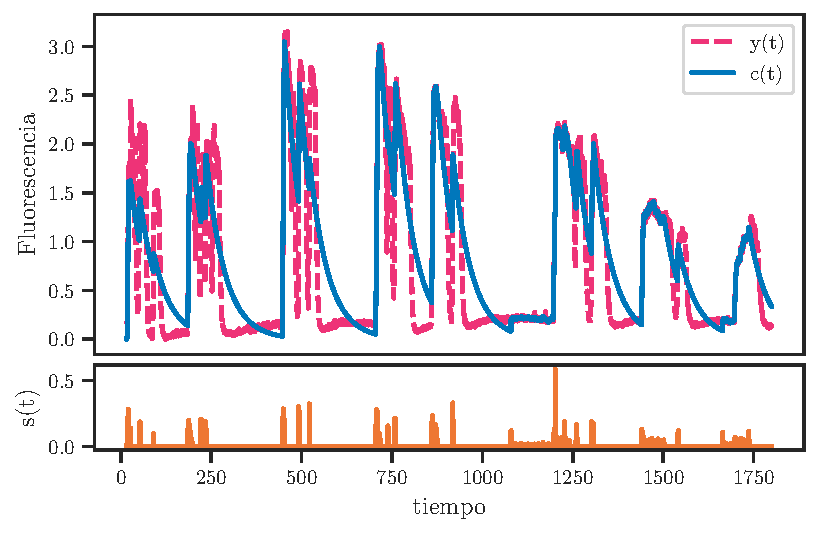
\includegraphics[width=\imsize]{oasis_p1.pdf}
 	\caption[Modelo autorregresivo generativo para la dinámica del calcio de la neurona AVAL.]{Modelo autorregresivo generativo para la dinámica del calcio de la neurona AVAL. El tren de spikes $s(t)$ se filtra para producir la traza de calcio $c(t)$; se utilizó $p = 1$ como orden del proceso AR. El ruido añadido por las mediciones produce la fluorescencia observada $y(t)$. }\label{f:oasis_p1}  
 \end{figure}
 
    \begin{figure}[h!]
 	\centering{}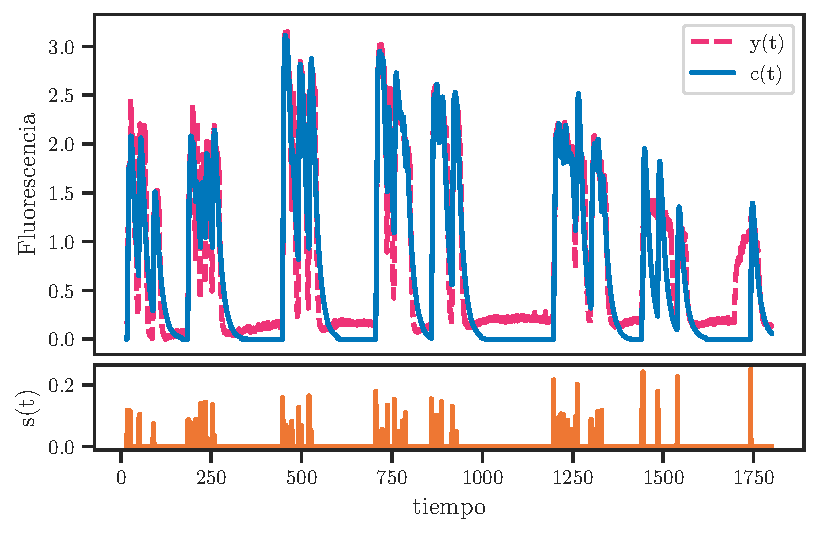
\includegraphics[width=\imsize]{oasis_p2.pdf}
 	\caption[Modelo autorregresivo generativo para la dinámica del calcio de la neurona AVAL.]{Modelo autorregresivo generativo para la dinámica del calcio de la neurona AVAL. El tren de spikes $s(t)$ se filtra para producir la traza de calcio $c(t)$; se utilizó $p = 2$ como orden del proceso AR. El ruido añadido por las mediciones produce la fluorescencia observada $y(t)$. }\label{f:oasis_p2}  
 \end{figure}
   
 Finalmente el marco AR tiene ciertas ventajas con respecto de los otros algoritmos estudiados en este apartado, como lo es el  permitir  un marco de modelado flexible e interpretable que conserva la trazabilidad computacional.   Además, los coeficientes AR se pueden estimar directamente a partir de los datos brutos de una manera completamente no supervisada, no requieren la existencia de spikes aislados para el ajuste fino de los distintos parámetros, y se pueden ajustar aún más durante el algoritmo de deconvolución \cite{pnevmatikakis_simultaneous_2016}. Aunque este marco AR(p) hace ciertas suposiciones simplificadoras sobre la linealidad y la dinámica del indicador de calcio, no obstante, da como resultado un estimador altamente eficiente desde el punto de vista computacional que alcanza un rendimiento de vanguardia entre los métodos no supervisados, como se ha demostrado  en Theis et al \cite{theis_benchmarking_2016}.
 
 \subsection{MCMC}
 
 Aunque el proceso de identificación de los parámetros AR del algoritmo OASIS suele ser muy útil para estimar la respuesta transitoria que surgiría de un solo spike, es útil refinar estas estimaciones dadas las estimaciones iniciales de los tiempos de spike. Para ello utilizamos  una extensión de los métodos Markov Chain Monte Carlo (MCMC) descritos en el \cref{sec:MCMC}. 
 
La \Cref{f:MCMC}(a) muestra la traza de calcio media obtenida con 500 muestras del algoritmo MCMC (azul) superpuesta a los datos reales (rosado), el método sigue  bastante bien la  traza de fluorescencia observada; el método MCMC puede modificar las constantes de tiempo inferidas para ajustarse mejor a los datos. Nótese que aquí el método MCMC se inicializó con los resultados obtenidos con el enfoque AR(2) explicado anteriormente. El método MCMC produce muestras de trenes de spikes con una resolución temporal continua y, por lo tanto, puede proporcionar más información sobre el número de spikes producidas en cada intervalo de tiempo y la incertidumbre de estas estimaciones debido al ruido y a la tasa de imagen finita. Esto se muestra en la \Cref{f:mcmc}, donde se traza la posterior marginal del número de spikes en cada intervalo de tiempo. Esta cuantificación de la incertidumbre temporal no está disponible con el algoritmo OASIS, que se basa en un marco de optimización convexa y, por lo tanto, proporciona una única estimación de la actividad neuronal, dividida en intervalos según la resolución de la tasa de imágenes.  El algoritmo predice la mayoría de los spikes ( \Cref{f:MCMC}c ) y proporciona estimaciones de baja varianza de los parámetros del modelo. Finalmente al comparar los metodos de deconvolución   AR(2)-MCMC (\Cref{f:MCMC}) obtiene mejores resultados que AR(2)-OASIS (\Cref{f:oasis_p2}). Ambos métodos superan al metodo  AR(1) (\cref{f:oasis_p1}), estableciendo que modelar el tiempo de subida puede mejorar significativamente la calidad de la deconvolución
 
 
 

    \begin{figure}[h!]
	\centering{}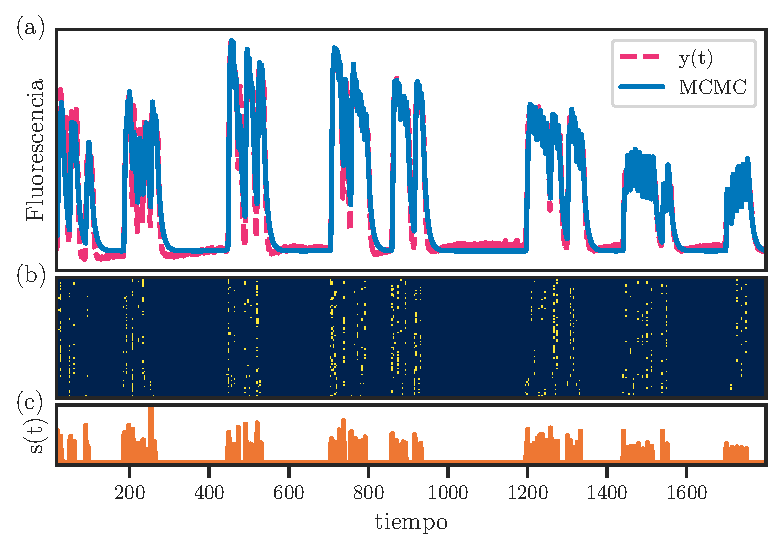
\includegraphics[width=\imsize]{MCMC.pdf}
	\caption[Aplicación del método MCMC.]{Aplicación del método MCMC. (a)  Datos de fluorescencia  de la neurona AVAL  y traza de fluorescencia reconstruida con  la  media de las muestras obtenida por el método MCMC completamente bayesiano con actualización de la constante temporal. El método MCMC  afina las constantes de tiempo para que se ajusten mejor a los datos observados.  (b)  Raster plot de los spikes de los  eventos del método MCMC. (c)  Actividad neuronal estimada  a partir de la media del marginal posterior por timebin con el método MCMC.  El método detecta con precisión los intervalos de bursting de las neuronas.  El método MCMC aunque más caro da una mejora significativa en la deconvolución de spikes comparado con el método OASIS. }\label{f:MCMC}  
\end{figure}


    \begin{figure}[h!]
	\centering{}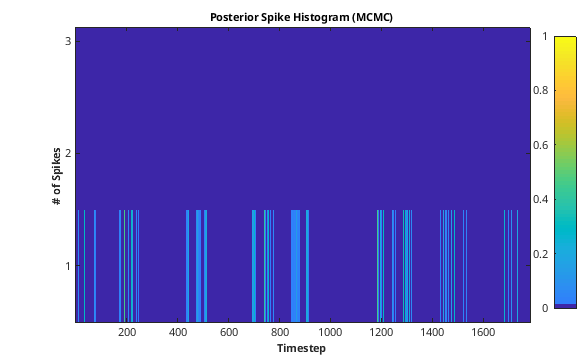
\includegraphics[width=\imsize]{mcmc.png}
	\caption[Aplicación del método MCMC.]{Representación codificada por colores del histograma marginal posterior empírico obtenido con el método MCMC. El mapa de colores muestra la probabilidad de un cierto número de spikes dentro de un timebin dado. El método MCMC puede cuantificar la incertidumbre e identificar múltiples spikes dentro de un mismo intervalo de tiempo.}\label{f:mcmc}  
\end{figure}

  
\subsection{Método de Kaplan  para detectar picos neuronales}

Aplicar diferencias finitas convencionales en los datos experimentales amplificará en gran medida cualquier ruido presente. La eliminación del ruido antes o después de la diferenciación no suele dar resultados satisfactorios. Un método que da buenos resultados es regularizar el propio proceso de diferenciación. Esto garantiza que la derivada calculada tendrá cierto grado de regularidad, hasta un punto que a menudo se puede controlar ajustando los parámetros. El marco que adoptaremos se encuentra en el \cref{C:ap1}. Sin embargo, el nivel y el tipo de regularización suelen imponerse de forma ad hoc, por lo que actualmente no existe un \textquote{mejor método} consensuado para obtener las derivadas \textquote{mejor ajustadas}. Para solventar este problema utilizamos un marco de optimización multiobjetivo para elegir los parámetros que equilibra dos métricas independientes.  Este enfoque minimiza una función de pérdida consistente en una suma ponderada de dos métricas calculadas a partir de la estimación de la derivada: la fidelidad de la integral de la derivada y su suavidad (\Cref{eq:ap:1}). Van breugel et al \cite{van_breugel_numerical_2020} sugieren estas métricas como aproximaciones para minimizar el error y el sesgo de la derivada estimada, y mostraron  que el barrido a través de los valores de un único hiperparámetro $\gamma$ produce estimaciones de la derivada que generalmente trazan el frente de Pareto de soluciones que minimizan el error y el sesgo. Es importante destacar que este marco de optimización no asume ningún conocimiento de la verdadera derivada subyacente y reduce la tarea de seleccionar muchos parámetros de cualquier algoritmo de diferenciación a la resolución de una función de pérdida con un único hiperparámetro. 

Para determinar un valor de $\gamma$  adecuada se utilizara  una heurística sencilla que es explicada en \cite{van_breugel_numerical_2020}  que se deriva del espectro de potencia y la resolución temporal de los datos. Todo este procedimiento se implementara  con el conjunto de herramientas Python de código abierto, pynumdiff.  Descubrimos que la mejor elección de $\gamma$ depende del contenido frecuencial de los datos.   En primer lugar, examinamos los espectros de potencia de los datos para elegir una frecuencia de corte que corresponda al inicio de la caída de potencia.  La \Cref{f:espectro_potencias_experimentos} muestra los espectros de potencia de los datos, indicando la frecuencia de corte (rojo) utilizada para seleccionar $\gamma$.  En cada conjunto de datos  la magnitud del ruido no cambia, esto se ve evidenciado  en que en un mismo experimento tanto los  espectro de potencias y la frecuencia de corte de las series neuronales son similares.  Esta frecuencia de corte, junto con la resolución temporal de los datos, se utilizan como entradas de la  heurística descrita por la \Cref{eq:84} para determinar un valor óptimo de $\gamma$.  

\begin{figure}[h!]
	\centering{}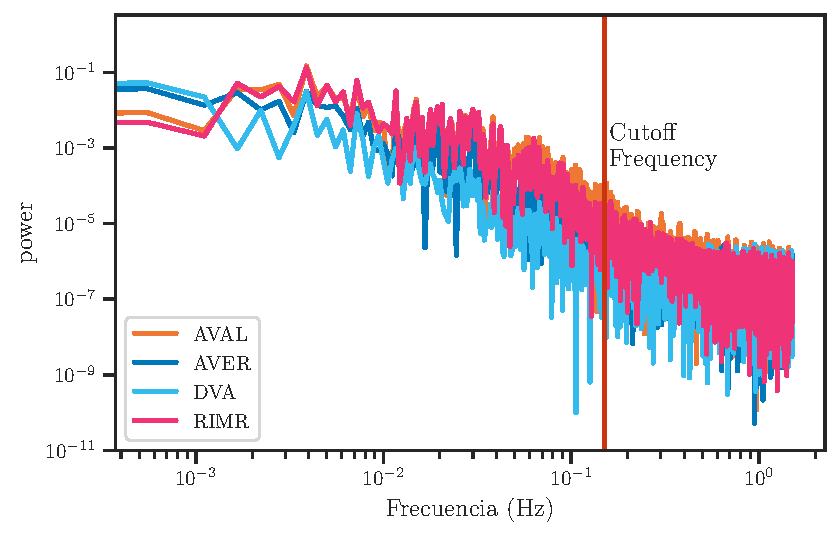
\includegraphics[width=\imsize]{espectro_potencias_experimentos.pdf}
	\caption[La frecuencia de los datos se evalúa inspeccionando los espectros de potencia; la línea roja indica la frecuencia utilizada para determinar $\gamma$]{La frecuencia de los datos se evalúa inspeccionando los espectros de potencia algunas neuronas de las series neuronales correspondientes a  los experimentos  Kaplan; la línea roja indica la frecuencia utilizada para determinar $\gamma$. }\label{f:espectro_potencias_experimentos}  
\end{figure}

Con $\gamma$ elegido, minimizamos nuestra función de pérdida de la \Cref{eq:ap:1} para encontrar los parámetros óptimos para la diferenciación numérica. La \Cref{f:resultado_picos}(naranja)   muestra  la derivada   de la serie temporal de la neurona AVAL de uno de los cinco gusanos de los experimentos de Kaplan \cite{kaplan_nested_2020}.   Habiendo encontrado  la derivada para inferir los spikes discretos utilizamos el método descrito en el \Cref{sec:metodos_picos}.   Este método depende de dos parámetros. En primer lugar, todos los métodos de detección de picos dependen en gran medida del grado de suavizado de los datos, que se logra en nuestro caso ajustando el hiperparámetro $\gamma$. En segundo lugar, la gama de deltas probados determina si este método tendrá éxito o no. Si el intervalo de deltas está dominado por deltas demasiado bajos o demasiado altos, no encontrará un punto de cambio adecuado, o el punto de cambio será demasiado liberal o demasiado conservador para todas las trazas. En este trabajo para determinar el rango delta  para una traza particular se utilizó la desviación estándar, estableciendo este valor como el máximo del rango delta, mientras que el mínimo y el intervalo entre deltas se establecían como la desviación estándar dividida por 100. La   \Cref{f:resultado_picos}(rosada) muestra los spikes inferidos por este método.




\begin{figure}[h!]
	\centering{}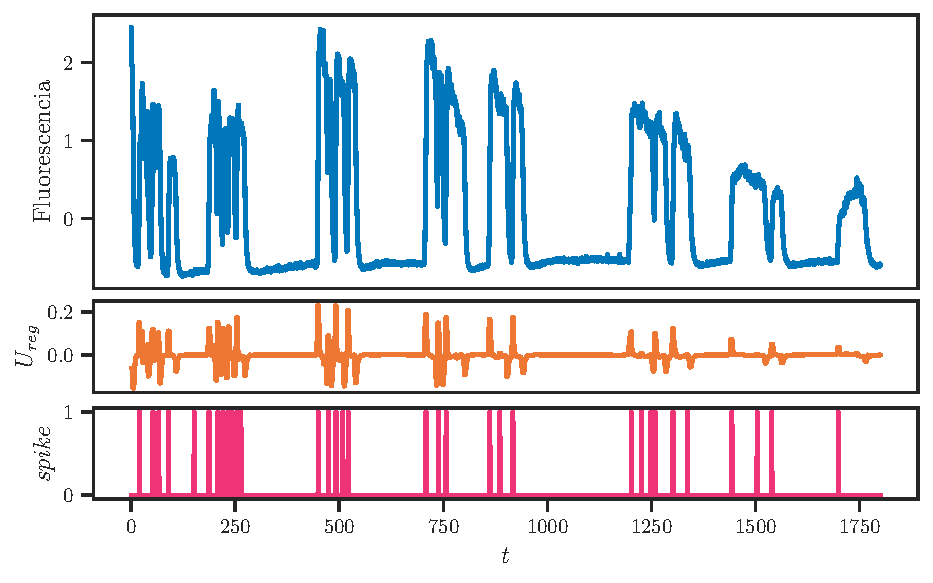
\includegraphics[width=\imsize]{kaplan_derivada.pdf}
	\caption[Inferencia de la actividad de spikes con el método de picos.]{Inferencia de la actividad de spikes con el método de picos.  trazas de calcio ($\Delta F/F$, azul), derivada regularizada (naranja) y spikes discretas inferidas de la derivada regularizada (rosado), se  destaca la eliminación de ruido a través de la inferencia de spikes.}\label{f:resultado_picos}  
\end{figure}




\subsection{CASCADE}

La idea clave en la que se basa este enfoque  de aprendizaje automático es que los datos de referencia (datos de entrenamiento) son tan importantes como el propio algoritmo y deben coincidir lo mejor posible con el nivel de ruido y la frecuencia de muestreo de los datos de imágenes de calcio de nuestros datos.  Para extraer los niveles de ruido, calculamos una métrica de ruido estandarizada $\nu$ que es robusta a los valores atípicos y aproxima la desviación estándar de las fluctuaciones de la línea de base de $\Delta F/F$
\begin{equation}
\nu = \frac{\text{Median}_t\left| \frac{\Delta F}{F}(t+1)-\frac{\Delta F}{F}(t) \right| }{\sqrt{f_r}},
\end{equation}

esta métrica se normalizó por la raíz cuadrada de la frecuencia de muestreo para permitir la comparación de las mediciones de ruido entre conjuntos de datos. En consecuencia, $\nu$ tiene unidades de  \unit{\percent \per\hertz^{-1/2}}.   La \Cref{f:nivel_ruido} muestra  el nivel de ruido $\nu$ en función del número de neuronas registradas simultáneamente en todos los experimentos considerados. Cada punto de datos representa un animal.  En el caso del conjunto de datos considerado en este apartado, el  nivel de ruido  promedio es de $1.52\pm0.45$  ( \unit{\percent \per\hertz^{-1/2}}; mediana $\pm$ s.d.) en 103 neuronas, el cual es un nivel de ruido bastante bajo. La  \Cref{f:histruido} muestra la distribución de ruido entre las neuronas de este conjunto de datos. En estas condiciones, se espera que las predicciones sean muy precisas por el algoritmo. 

    \begin{figure}[h!]
	\centering{}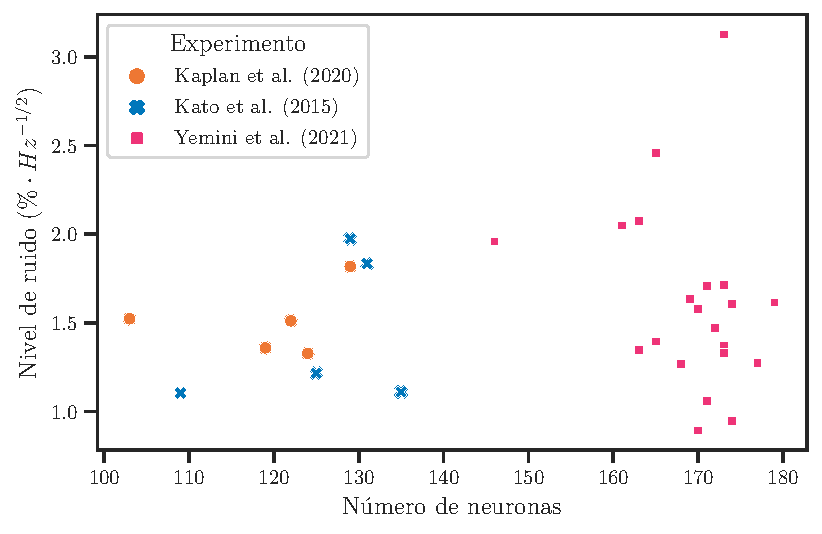
\includegraphics[width=\imsize]{nivel_ruido.pdf}
	\caption[Número de neuronas registradas en función de los niveles de ruido estandarizados.]{Número de neuronas registradas en función de los niveles de ruido estandarizados (en \unit{\percent \per\hertz^{-1/2}}) para todos los experimentos.}\label{f:nivel_ruido}  
\end{figure}



    \begin{figure}[h!]
	\centering{}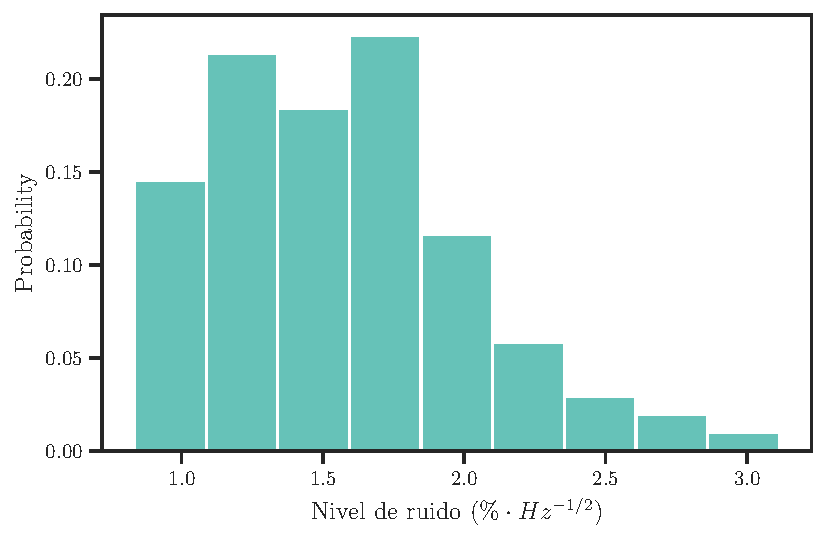
\includegraphics[width=\imsize]{histograma_ruido.pdf}
	\caption[Histograma de los niveles de ruido entre las neuronas]{Histograma de los niveles de ruido entre las neuronas
}\label{f:histruido}  
\end{figure}

A continuación, se buscó    el modelo preentrenado  de CASCADE que mejor se adapte a los datos. En nuestro caso como no tenemos una verdad fundamental específica para el conjunto de datos,  utilizamos un modelo que ha sido entrenado en todos los conjuntos de datos disponibles (llamado \textquote{Modelo Global EXC}).   Este modelo está entrenado en un conjunto de datos de verdad fundamental remuestreado. El conjunto de datos de entrenamiento se remuestrea a la frecuencia de muestreo deseada y a múltiples niveles de ruido. El modelo elige automáticamente el modelo con los niveles de ruido coincidentes para cada neurona. Solo se tiene  que seleccionar la frecuencia de muestreo correcta (que se indica en el nombre del modelo). En nuestro caso la frecuencia de muestro es \qty{3}{\hertz}.  Ademas existen  dos especificaciones del modelo adicionales que se pueden elegir: núcleos \textquote{causales} y \textquote{suavizados}.  El mas adecuado a nuestros datos es el núcleo casual ya que   la actividad de spikes se asigna casi exclusivamente a puntos de tiempo posteriores al inicio del evento de calcio. 

Por lo tanto utilizando el modelo   \textbf{ Global EXC 3Hz smoothing400ms causalkernel}, estimamos las tasas de spikes  de las 103 neuronas. La \Cref{f:cascade_spikes} destaca cómo el algoritmo de inferencia de spikes puede eliminar el ruido de las trazas de calcio. Esto se puede observar comparando las trazas de calcio sin procesar (azul) con las tasas de spikes inferidas (naranja). Las tasas de spikes inferidas son mucho más suaves y menos ruidosas que las trazas de calcio sin procesar. Para obtener eventos de spikes discretos a partir de las probabilidades inferidas, se aplicó un umbral para binarizar estas probabilidades. Se encontró que un umbral de $0.4$ es adecuado para realizar una buena discretización. El resultado se muestra en el rasterplot de la \Cref{f:cascade_spikes}, en donde se evidencia que los tiempos de los spike  estan sincronizados con  la dinámica de la neurona.

    \begin{figure}[h!]
	\centering{}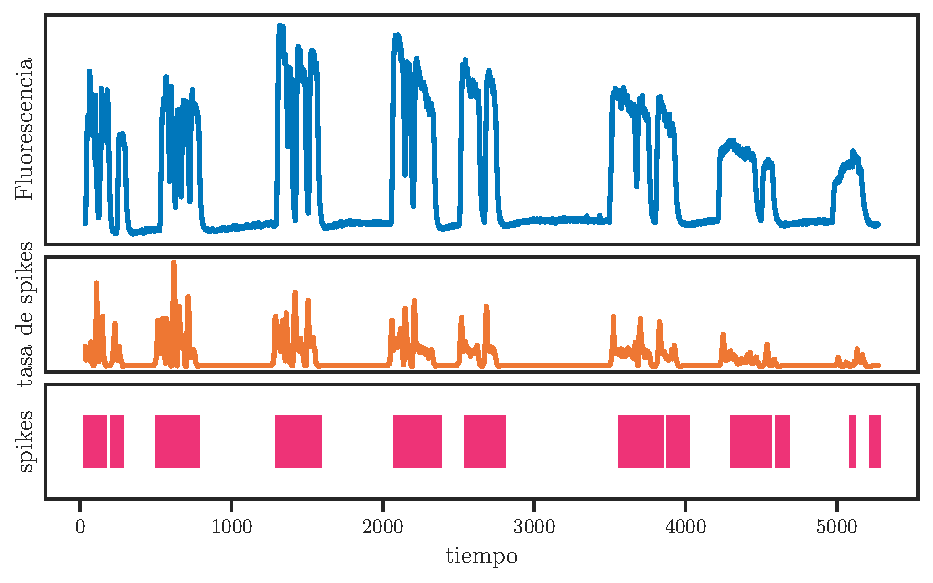
\includegraphics[width=\imsize]{cascade_spikes.pdf}
	\caption[Inferencia de la actividad de spikes con CASCADE.]{Inferencia de la actividad de spikes con CASCADE.  trazas de calcio ($\Delta F/F$, azul), tasas de spikes inferidas (naranja) y spikes discretas inferidas (rosado), se  destaca la eliminación de ruido a través de la inferencia de spikes.}\label{f:cascade_spikes}  
\end{figure}

Ademas los datos $\Delta F/F$ sin procesar a menudo también presentaban ruido correlacionado, visible como una franja vertical ruidosa en los gráficos de matriz, que era pequeño para las neuronas individuales pero tendía en algunos conjuntos de datos a dominar el $\Delta F/F$ medio entre las neuronas, posiblemente debido al ruido técnico. CASCADE eliminó visiblemente estos artefactos (\Cref{f:cascade_2}). Este ejemplo ilustra cómo la inferencia de spikes calibrada por CASCADE puede aplicarse para eliminar el ruido de las señales de calcio y para analizar la estructura temporal de la dinámica de las poblaciones neuronales. 


    \begin{figure}[h!]
	\centering{}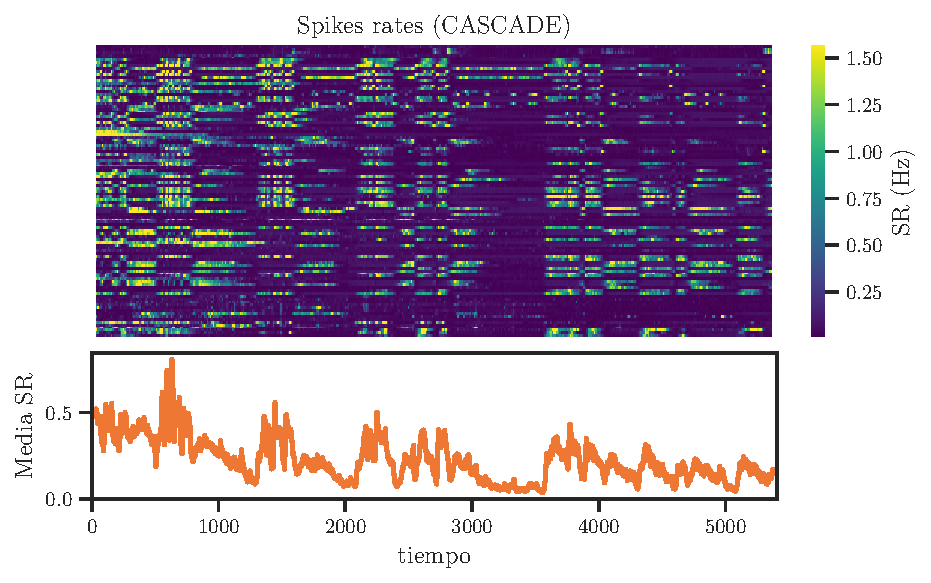
\includegraphics[width=\imsize]{cascade_2.pdf}
	\caption[Tasas de spikes inferidas con CASCADE  del conjunto de datos RIShisCl  (gusano 1).]{Tasas de spikes inferidas con CASCADE  del conjunto de datos RIShisCl  (gusano 1). El ruido se redujo por parte del algoritmo.}\label{f:cascade_2}  
\end{figure}

  
\subsection{Patrones de actividad neuronal observados}


Se utilizaron los anteriores algoritmos   para inferir los spikes de las 103 neuronas registradas simultáneamente del gusano 1 del conjunto de datos RIShisCl del experimento de Kaplan.  La \Cref{f:cascade_1} muestra las señales de calcio  sin procesar. Las franjas verticales recurrentes visibles a nivel global  marcan la presencia de actividad de red correlacionada, en consonancia con la presencia de oscilaciones colectivas  (estados ascendentes y descendentes) que se sabe que ocurren en diversas circunstancias en la dinámica neuronal espontanea. 


    \begin{figure}[h!]
	\centering{}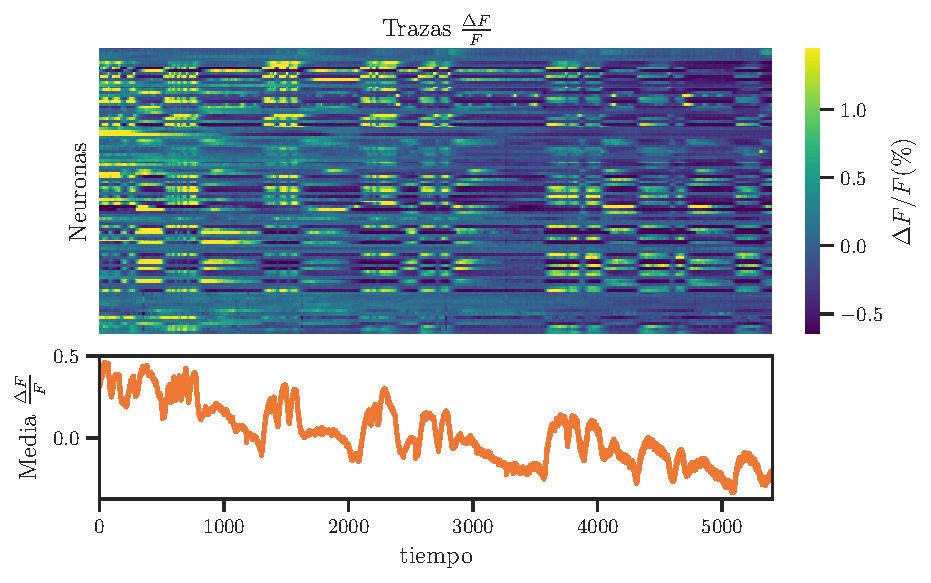
\includegraphics[width=\imsize]{cascade_1.pdf}
	\caption[Trazas $\Delta F/F$ sin procesar  del conjunto de datos RIShisCl  (gusano 1).]{Trazas $\Delta F/F$ sin procesar  del conjunto de datos RIShisCl  (gusano 1).  Las franjas verticales recurrentes visibles a nivel global  marcan la presencia de actividad de red correlacionada.}\label{f:cascade_1}  
\end{figure}



Al aplicar los algoritmos anteriormente descritos se obtienen los resultados mostrados en las \Cref{f:oasis_spike,f:MCMC_spike,f:kaplan_raster,f:cascade}.   El algoritmo OASIS (\Cref{f:oasis_spike}) muestra claras diferencias en la actividad de red correlacionada  con respecto a las  trazas de fluorescencia    (\Cref{f:cascade_1}). Esto puede deberse a que el algoritmo no hace una inferencia a nivel poblacional y por tanto puede ser sensible  a artefactos de ruido de neuronas individuales que hace que parte de la sincronización a nivel temporal se pierda.  En el caso de el algoritmo MCMC (\Cref{f:MCMC_spike})  el resultado es mas consistente con la dinámica	 real de los datos, esto se debe a que este algoritmo  realiza muestreos estocásticos aumentando la calidad de la inferencia, la desventaja de este tipo de algoritmos es su alto costo computacional. Por otro lado el método de Kaplan (\Cref{f:kaplan_raster}) muestra una característica deseable de los spikes la  escasez de picos (spike sparsity) de la actividad neuronal, el problema es que algunas dinámicas de baja frecuencia pueden perderse por este método.   Finalmente  en comparación con los otros enfoques, las predicciones de spikes  de CASCADE fueron más precisas (\Cref{f:cascade}). Se logro encontrar la presencia de actividad de red correlacionada tal como en los datos reales.   La comparación de las señales $\Delta F/F$ y  los spikes inferidos mostró que CASCADE detectó fases de actividad, pero suprimió de forma efectiva las fluctuaciones irregulares pequeñas en las trazas de actividad, lo que indica que la inferencia de spikes suprimió el ruido. 

 \begin{figure}[h!]
	\centering{}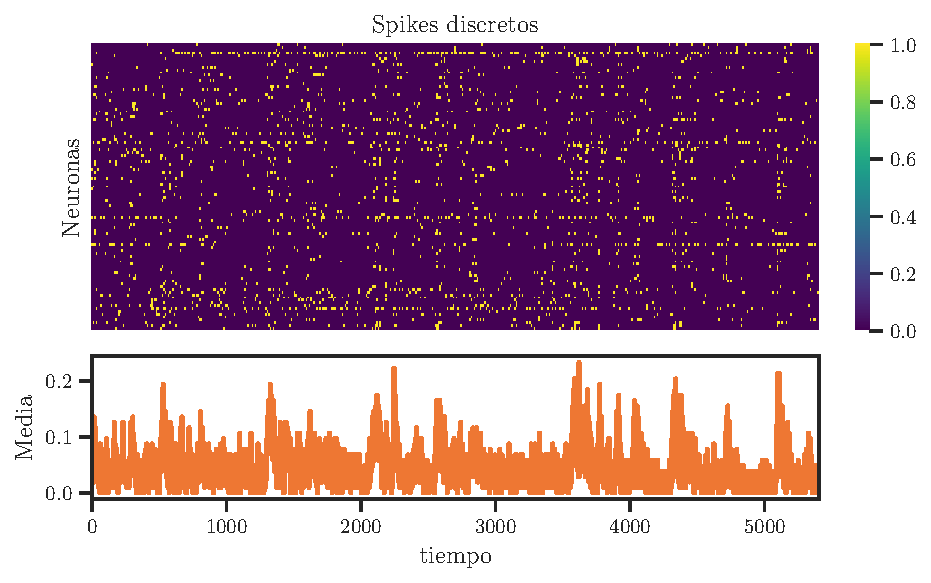
\includegraphics[width=\imsize]{oasis_spike.pdf}
	\caption[Representación  matricial de los spikes de las 103 neuronas obtenidas con OASIS. ]{Representación  matricial de los spikes de las 103 neuronas obtenidas con OASIS.}\label{f:oasis_spike}  
\end{figure}

\begin{figure}[h!]
	\centering{}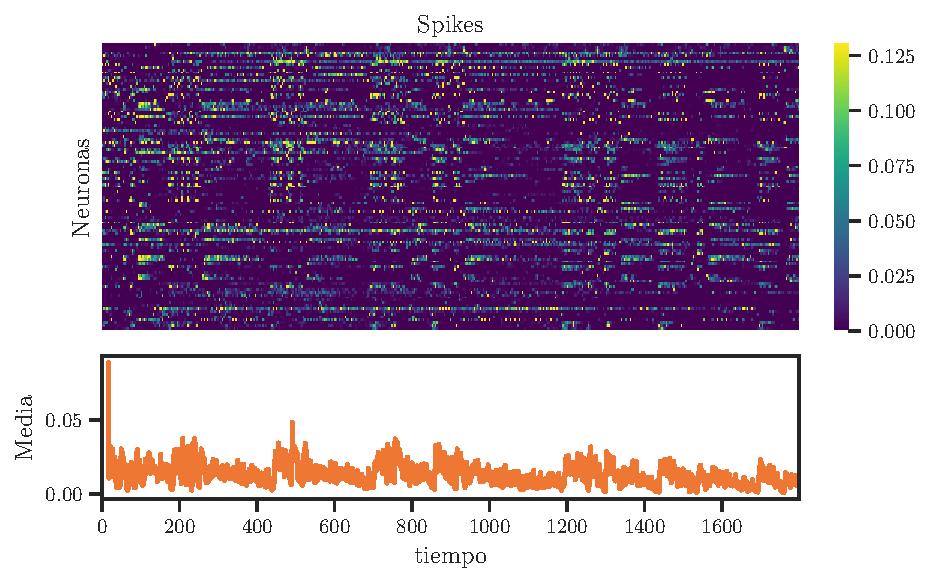
\includegraphics[width=\imsize]{MCMC_spike.pdf}
	\caption[Representación  matricial de los spikes de las 103 neuronas obtenidas con MCMC. ]{Representación  matricial de los spikes de las 103 neuronas obtenidas con MCMC. La matriz muestra  actividades correlacionadas en la red (que aparecen como alineaciones verticales de spikes).}\label{f:MCMC_spike}  
\end{figure}


\begin{figure}[h!]
	\centering{}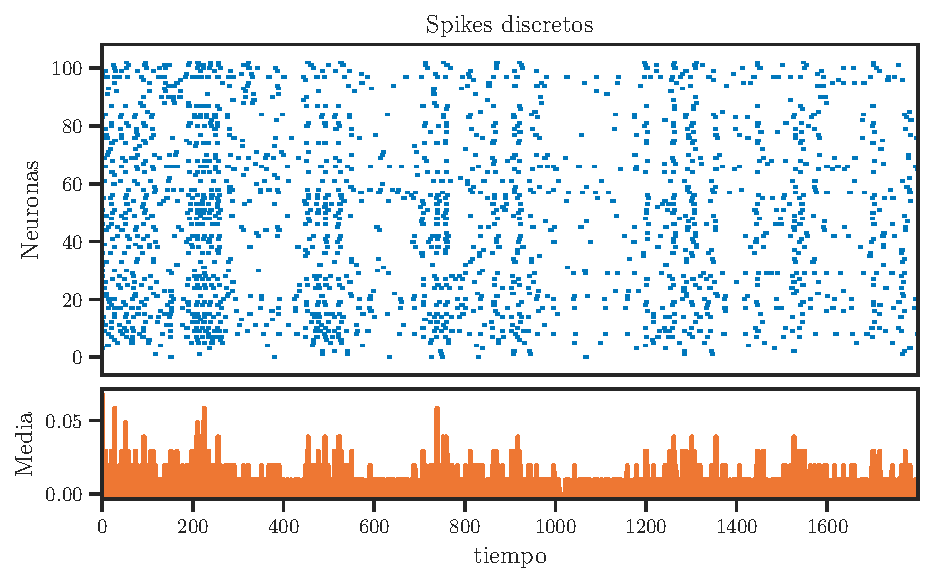
\includegraphics[width=\imsize]{kaplan_raster.pdf}
	\caption[Representación  matricial de los spikes de las 103 neuronas obtenidas con el método de Kaplan et al. ]{Representación  matricial de los spikes de las 103 neuronas obtenidas con el método de Kaplan et al. La matriz muestra  actividades correlacionadas en la red (que aparecen como alineaciones verticales de spikes).}\label{f:kaplan_raster}  
\end{figure}

\begin{figure}[h!]
	\centering{}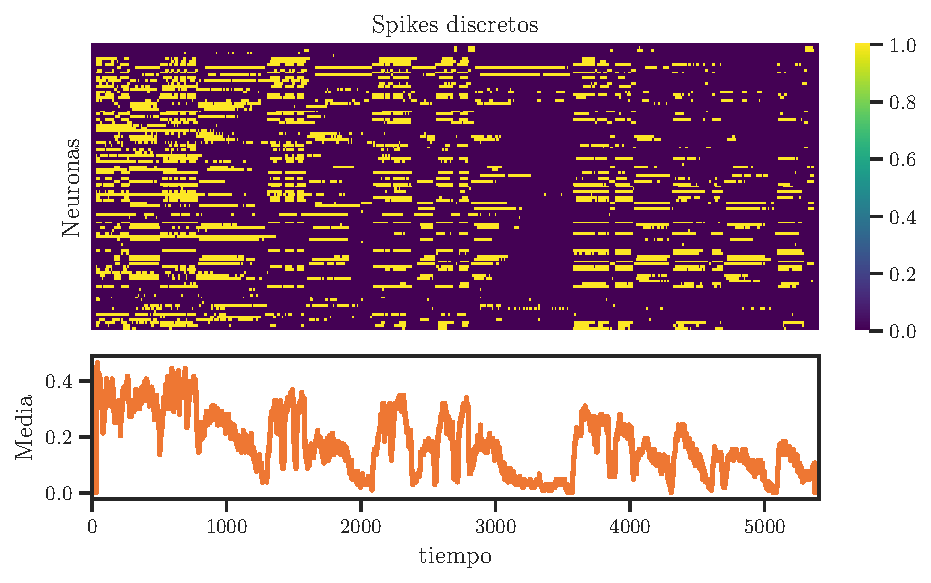
\includegraphics[width=\imsize]{cascade_3.pdf}
	\caption[Representación  matricial de los spikes de las 103 neuronas obtenidas con CASCADE. ]{Representación  matricial de los spikes de las 103 neuronas obtenidas con CASCADE. La matriz muestra  actividades correlacionadas en la red (que aparecen como alineaciones verticales de spikes).}\label{f:cascade}  
\end{figure}



\subsection{Discusión}

Estamos interesados en los grupos de neuronas coactivos y contiguos. Para ello, primero buscamos inferir  la actividad de cada una de las neuronas umbralizando las fluctuaciones de intensidad de fluorescencia $\Delta F/F$.  Para realizar esta umbralizacion  nos basamos  en tres algoritmos disponibles en la literatura: métodos auto-regresivos AR(p), métodos de inferencia bayesiana y métodos de aprendizaje profundo.  Los enfoques bayesianos  (MCMC)   superaron a los métodos auto-regresivos AR(p)  (OASIS) tanto en la estimación de tasas de spike como en la actividad global de red coordinada. Curiosamente, el algoritmo MCMC  devuelve trenes de spikes de muestra reales que pueden utilizarse, por ejemplo, para investigar las propiedades de la red en función de los tiempos de los spikes. Al mismo tiempo, MCMC devuelve muchos de estos trenes de spikes, muestreados según la distribución de probabilidad posterior, lo que permite tanto la estimación de las probabilidades de spikes como una indicación del nivel de incertidumbre de la estimación \cite{deneux_accurate_2016}. 

CASCADE funcionó mejor que todos los demás métodos en la mayoría de los casos. El método  puede inferir  los spikes con alta precisión, incluso a niveles de SNR bajos. Esto sugiere que CASCADE puede utilizarse para analizar datos de imágenes de calcio de poblaciones muy grandes de neuronas. Por lo que  en comparación con los otros enfoques estudiados en este apartado, las predicciones de la actividad global correlacionada   de CASCADE fueron más precisas, pero también menos sesgadas hacia subestimaciones de los spikes reales tal como el algoritmo OASIS (\Cref{f:oasis_spike}). En segundo lugar, dado que no se  necesita ajustar los hiperparámetros, la aplicación de la inferencia de spikes se vuelve sencilla en la práctica. Estos resultados sugieren que CASCADE es un método robusto y confiable para la inferencia de spikes en una amplia gama de condiciones experimentales. Por lo tanto en conjunto, estos aspectos reflejan que, a diferencia de los algoritmos basados en modelos, CASCADE puede hacer uso de conjuntos de datos de referencia de manera eficiente y natural. Por lo que en el resto de este documento utilizamos CASCADE para  la inferencia de los spikes de la  dinámica global de todos los experimentos.

  
 
 \section{Clústeres de actividad neuronal}\label{sec:actividad_neuronal_experimento}
 
 
 
En este apartado, caracterizamos los patrones espaciales de la actividad neuronal colectiva calculando el número de clústeres y su distribución de tamaños (número de activaciones; ver \cref{sec:clusteres}) en los datos experimentales. Estudiamos las estadísticas de los clústeres en el marco de la teoría de la percolación. Como se discutió en el \cref{sec:cap-percolacion}, la percolación describe el comportamiento de los clústeres en un grafo y cómo cambian los tamaños de los clústeres con el número de unidades activas, pasando de pequeños clústeres a la aparición de un gran clúster más allá de un nivel crítico de actividad \cite{rocha_recovery_2022}. A lo largo de este estudio, analizamos la actividad espontánea.
 
 \subsection{Correlación entre actividades neuronales}\label{sec:correlacion}
 
 Antes de abordar la caracterización de los clústeres neuronales de la actividad neuronal de los experimentos con C. elegans vamos a detallar varias características destacadas en estas series temporales. Para visualizar mejor los grupos de neuronas que comparten actividad en  las series temporales, se aplico a los conjuntos de datos un algoritmo de clustering jerárquico/aglomerativo mediante la función de seaborn  \textbf{clustermap}\footnote{https://seaborn.pydata.org/generated/seaborn.clustermap.html} (  \Cref{fig:seriedatos}).  En primer lugar, existen grupos de neuronas  que mostraron activación e inactivación sincronizadas. Dado que no existe estimulación en los datos de Kaplan et al. y Kato et al. este comportamiento se considera como  actividades espontáneas. Estas observaciones son consistentes con lo reportado por Kat et al. \cite{kato_global_2015}. Para aclarar aún más esto, se determinaron las correlaciones cruzadas en las actividades neuronales utilizando el metodo de correlación de Pearson 
 en todas las combinaciones de neuronas por pares (\Cref{fig:correlaciones_experimentos}). Se observó que el tamaño de cada grupo correlacionado difería considerablemente entre los distintos conjuntos de datos. Aquí, también es evidente que en muchos casos, en cada conjunto  hay al menos un grupo principal de neuronas con actividad correlacionada, y a menudo hay otro grupo correlacionado que está correlacionado negativamente con el primer grupo. Al detallar las  neuronas miembro por ejemplo en el conjunto de Yemini et al se revela que estos grupos corresponden a los grupos bien conocidos de neuronas relacionadas con los movimientos de retroceso y avance de los animales, a saber, las neuronas AVA, AVE y RIM, etc. en el primer grupo (las correlaciones son por ejemplo: (AVAR,AVAL): 0.942, (AVAL,AVER): 0.8941, (AVAL,RIMR): 0.8911 ), y las neuronas RIB, RID y RME, etc. en el segundo grupo ((RIBL,RID): 0.918, (RIBL,RMEL): 0.5181, (RID,RMER): 0.46). Otros grupos que se correlacionaron entre los datos incluyeron  [(OLLL,OLLR): 0.96, (OLLL,OLQDL): 0.82, (OLQDL, OLQDR): 0.582 ]  y [(I2L,I2R): 0.97, (I2L,MCL): 0.9963, (I2R,MCL): 0.971]     , y  [(BAGL,BAGR): 0.72, (RIAL,RIAR): 0.52, (RMDVL,RMDVR): 0.667, (SMDDL,SMDDR): -0.51] \cite{toyoshima_deducing_2022}. Es importante destacar  que la correlación entre la actividad de estos grupos era consistente en diferentes muestras de gusanos de los distintos experimentos.
 

 
  \begin{figure}
 	\centering
 	\begin{subfigure}[b]{0.3\textwidth}
 		\centering
 		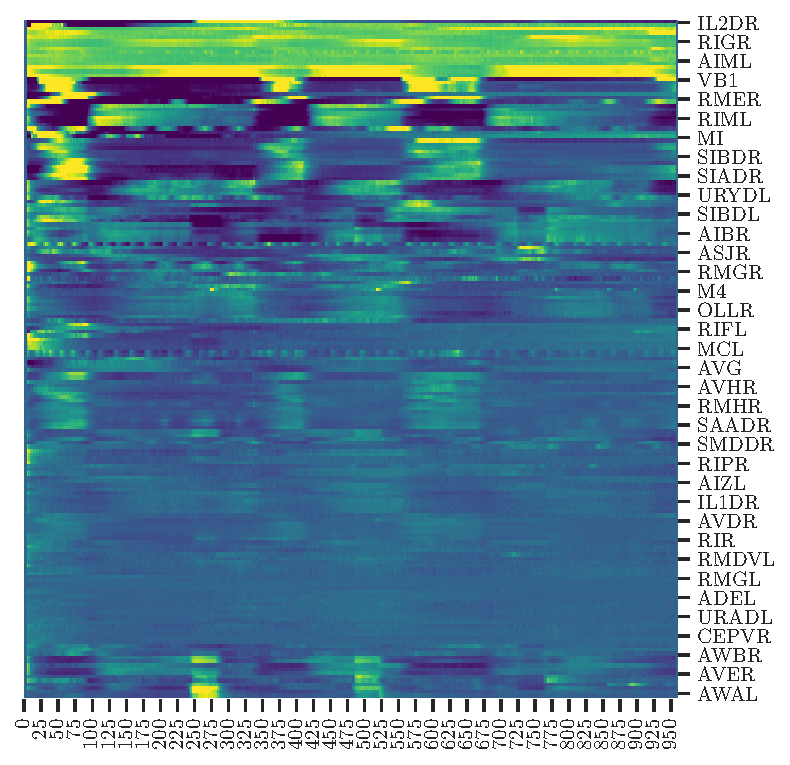
\includegraphics[width=\textwidth]{cluster_neuropal.pdf}
 		\caption{}
 		\label{fig:cluster_neuropal}
 	\end{subfigure}
 	\begin{subfigure}[b]{0.3\textwidth}
 		\centering
 		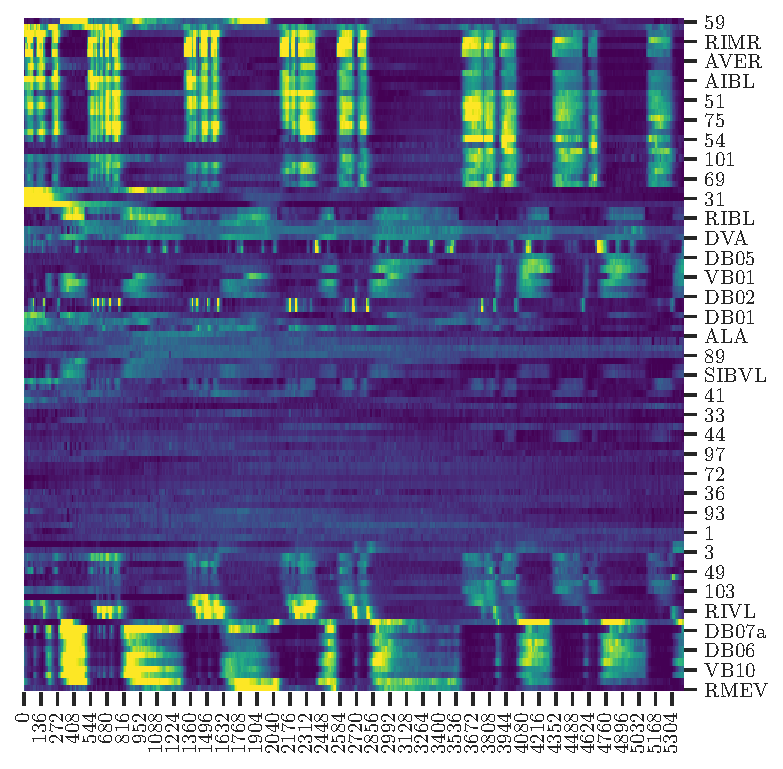
\includegraphics[width=\textwidth]{cluster_kaplan.pdf}
 		\caption{}
 		\label{fig:cluster_kaplan}
 	\end{subfigure}
 	\begin{subfigure}[b]{0.3\textwidth}
 		\centering
 		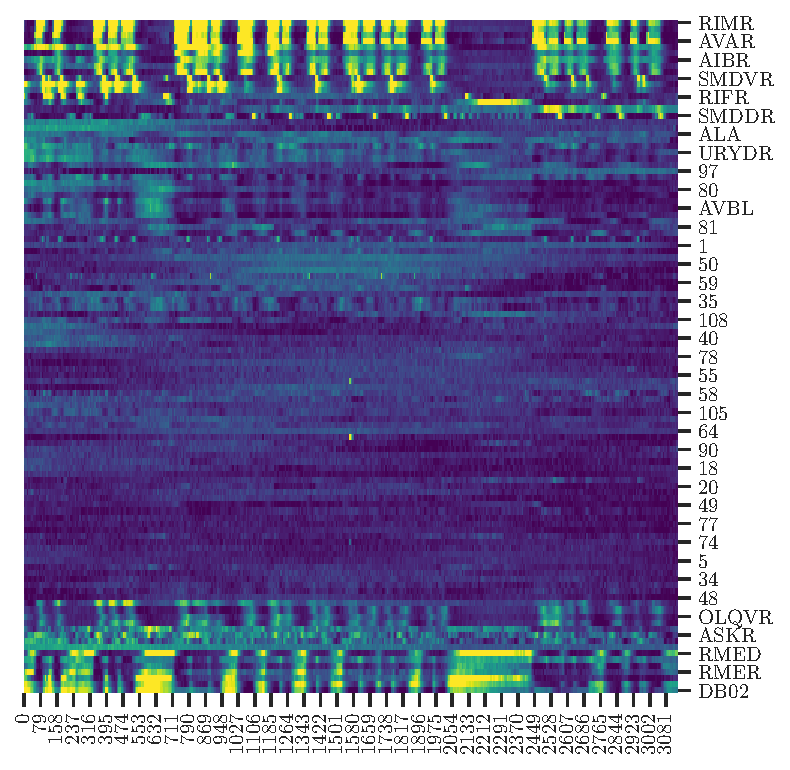
\includegraphics[width=\textwidth]{cluster_kato.pdf}
 		\caption{}
 		\label{fig:cluster_kato}
 	\end{subfigure}
 	\caption[Serie temporal de actividad de las neuronas del primer gusano en cada conjunto de datos.]{ Serie temporal de actividad de las neuronas del primer gusano en cada conjunto de datos. Cada fila representa una neurona, cuyo orden se determinó mediante agrupamiento jerárquico. (a) Yemini et al. (b) Kaplan et al. (c) Kato et al.}\label{fig:seriedatos}
 \end{figure}
 
 \begin{figure}[h!]
\centering
 	 	\begin{subfigure}[b]{0.3\textwidth}
	\centering
	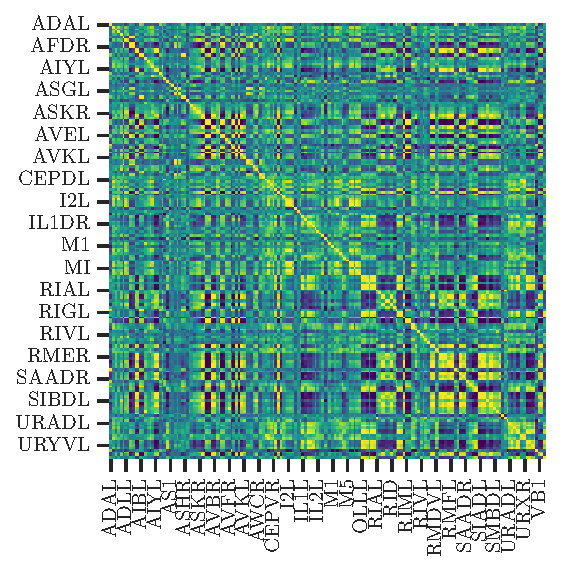
\includegraphics[width=\textwidth]{correlacion_neuropal.pdf}
	\caption{}
	\label{fig:correlacion_neuropal}
\end{subfigure}
\begin{subfigure}[b]{0.3\textwidth}
	\centering
	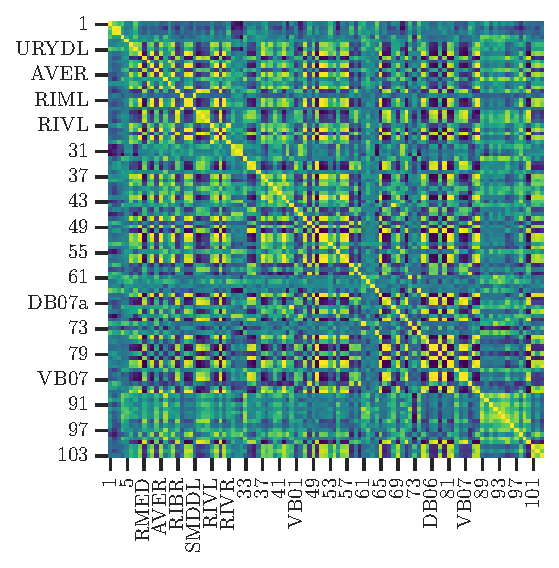
\includegraphics[width=\textwidth]{correlacion_kaplan.pdf}
	\caption{}
	\label{fig:correlacion_kaplan}
\end{subfigure}
\begin{subfigure}[b]{0.3\textwidth}
	\centering
	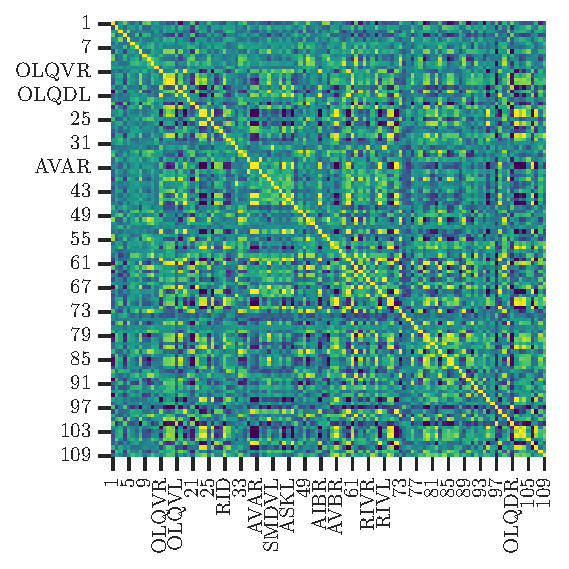
\includegraphics[width=\textwidth]{correlacion_kato.pdf}
	\caption{}
	\label{fig:correlacion_kato}
\end{subfigure}
\caption[Correlación cruzada por pares de las actividades de las neuronas  del primer conjunto de datos de los experimentos con C elegans.]{Correlación cruzada por pares de las actividades de las neuronas  del primer conjunto de datos de los experimentos con C elegans. (a)  Yemini et al. (b) Kaplan et al. (c) Kato et al. El color amarillo muestra una correlación positiva y el color azul muestra una correlación negativa.} \label{fig:correlaciones_experimentos}
 \end{figure}
 
 
 

 
 
 
 \subsection{Calculo de distribución de clústeres red cuadrada}\label{eq:redcuadarda_clusteres}
 
 Antes de encontrar la distribución de los tamaños de los clústeres de los datos experimentales,   corroboraremos el buen funcionamiento del algoritmo  descrito en el  \cref{sec:alg_cluster}. Para este fin,  utilizaremos la red cuadrada como  modelo de control.  La ventaja de este modelo es que tanto la   distribución de clústeres  y sus propiedades estadísticas están disponibles  en la literatura, por lo que podemos compararlos con los resultados del  algoritmo.   Generamos  una red de puntos $L\times L$ que están ocupados con probabilidad $p$.   La matriz resultante se ilustra en la \Cref{f:matriz_clusteres}(a). Sin embargo, esta visualización no nos proporciona ninguna información sobre la conectividad de los sitios en este sistema. En su lugar, analizamos las regiones conectadas en el sistema. Para encontrar las regiones conectadas utilizamos el algoritmo descrito en el  \cref{sec:alg_cluster}. Tanto para este ejemplo como para los resultados experimentales y el modelo  de criticidad neuronal utilizamos la funcion de Scipy \textbf{sparse.csgraph.connected\_components}\footnote{\url{https://docs.scipy.org/doc/scipy/reference/generated/scipy.sparse.csgraph.connected_components.html}} para analizar los componentes conectados de un grafo cuya entrada es  la matriz de adyacencia del grafo.  Ademas como deseamos calcular las componentes débilmente conexas utilizamos el valor \textquote{weak} del parámetro  connection. 
 
 \begin{figure}[h!]
 	\centering{}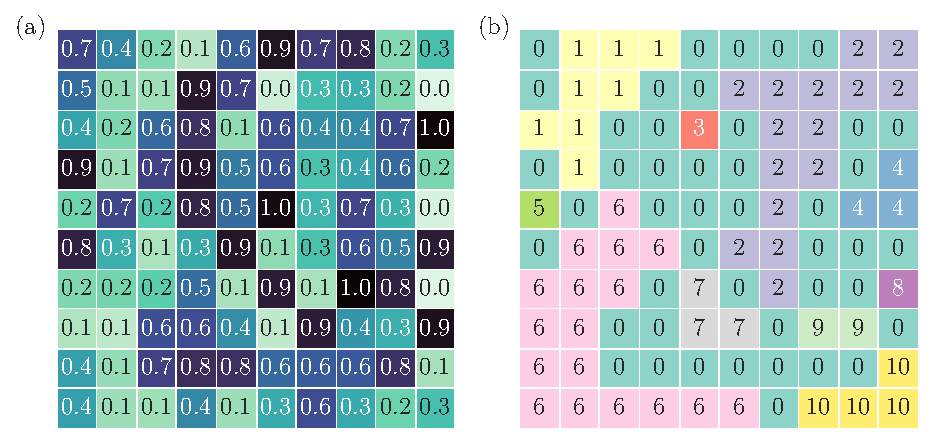
\includegraphics[width=\imsize]{matriz_clusteres.pdf}
 	\caption[ Ilustración de una matriz de números aleatorios de $10\times10$, y los diversos sitios establecidos para $p=0.45$. ]{ Ilustración de una matriz de números aleatorios de $10\times10$, y los diversos sitios establecidos para $p=0.45$. (a) Ilustración de una matriz de números aleatorios de $10\times10$ . (b) Ilustración de la matriz de índices  para $p = 0.45$.}\label{f:matriz_clusteres}  
 \end{figure}

 Esta función devuelve la matriz de etiquetas, que para cada nodo en la matriz de adyacencia original indica a qué clúster pertenece. Los clústeres se numeran secuencialmente y a cada clúster se le asigna un índice. Todos los nodos con el mismo índice pertenecen al mismo clúster. La matriz resultante se muestra en la \Cref{f:matriz_clusteres}(b), donde se muestra el índice para cada sitio y se utiliza un color para indicar los diversos clústeres. 
 
 \subsubsection{Distribución del numero de clústeres}
 
  Para comprender mejor la distribución de los tamaños de los clústeres, estudiemos la \Cref{f:matriz_clusteres} con más detalle.  Hay 3 clústeres de tamaño $s = 1$, un clúster de tamaño $s = 2$, 2 clústeres de tamaño $s=3$ y 1 clústeres de tamaño $s=4$, $s=8$, $s=15$ y $s=17$ respectivamente.   Tal como se describió en el \Cref{sec:medicion_clusteres}  
mediante  un histograma de tamaños de clústeres podemos encontrar la distribución de clústeres numéricamente.  Para los clústeres en la  \Cref{f:matriz_clusteres}   la estimación de $\overline{n(s, p;L)}$ (\Cref{eq:88}) basada en esta única realización se resume  en el \cref{table:histograma_cluster}. 
 \begin{table}[h!]
	\centering
	\caption[Histograma de tamaños de clústeres]{ Histograma de tamaños de clústeres.}
	\begin{tblr}{colspec={llllllll},
			row{odd} = {bg=gray8},
			row{even} = {bg=gray9},
			column{1} = {bg=red3, fg=white, font=\sffamily},
		}
		
		$s$ & 1 & 2 & 3 & 4 &     8 &15 & 17 \\
		$Ns$ & 3 & 1 & 2 & 1 &   1 & 1  & 1\\
		$n(s,p)$ & 3/100 & 1/100 & 2/100 & 1/100   & 1/100 &  1/100 &  1/100\\
	\end{tblr}
	\label{table:histograma_cluster}
\end{table}

Teniendo en cuenta lo anterior se simulo una red cuadrada con  $L=1000$. Para producir buenas estimaciones estadísticas de $n(s, p)$ se realizaron $M=1000$  realizaciones aleatorias del sistema. Estimamos $\overline{n(s, p; L)}$ utilizando la  \Cref{eq:88} para $p=0.57$, el resultado se muestra en la  \Cref{f:num_clusteres_red_cuadrada}a,b.    Desafortunadamente, este gráfico no es muy útil. El problema es que hay muchos valores de $s$ para los que tenemos pocos o ningún dato. Para los valores pequeños de $s$ tenemos muchos clústeres para cada valor de $s$ y las estadísticas son buenas. Pero para los valores grandes de $s$, tenemos menos de un punto de datos para cada valor de $s$. Por lo tanto, nuestra distribución medida $\overline{n(s, p; L)}$ es una mala representación de la $n(s, p; L)$ real en este rango.

El problema con los resultados medidos en la  \Cref{f:num_clusteres_red_cuadrada}a,b ocurre porque hemos elegido un tamaño de bin muy pequeño para el histograma. Sin embargo, vemos que para valores pequeños de $s$ queremos tener un tamaño de bin pequeño, ya que las estadísticas aquí son buenas, pero para valores grandes de $s$ queremos tener tamaños de bin más grandes. Esto a menudo se resuelve utilizando un binning logarítmico.  El gráfico resultante  se muestra en la \Cref{f:num_clusteres_red_cuadrada}c. Observase que el gráfico resultante ahora es mucho más fácil de interpretar que el gráfico binneado linealmente.  Por lo tanto, en lo siguiente adaptaremos estrategias de binning logarítmico siempre que midamos un conjunto de datos que es escaso.



\begin{figure}[h!]
	\centering{}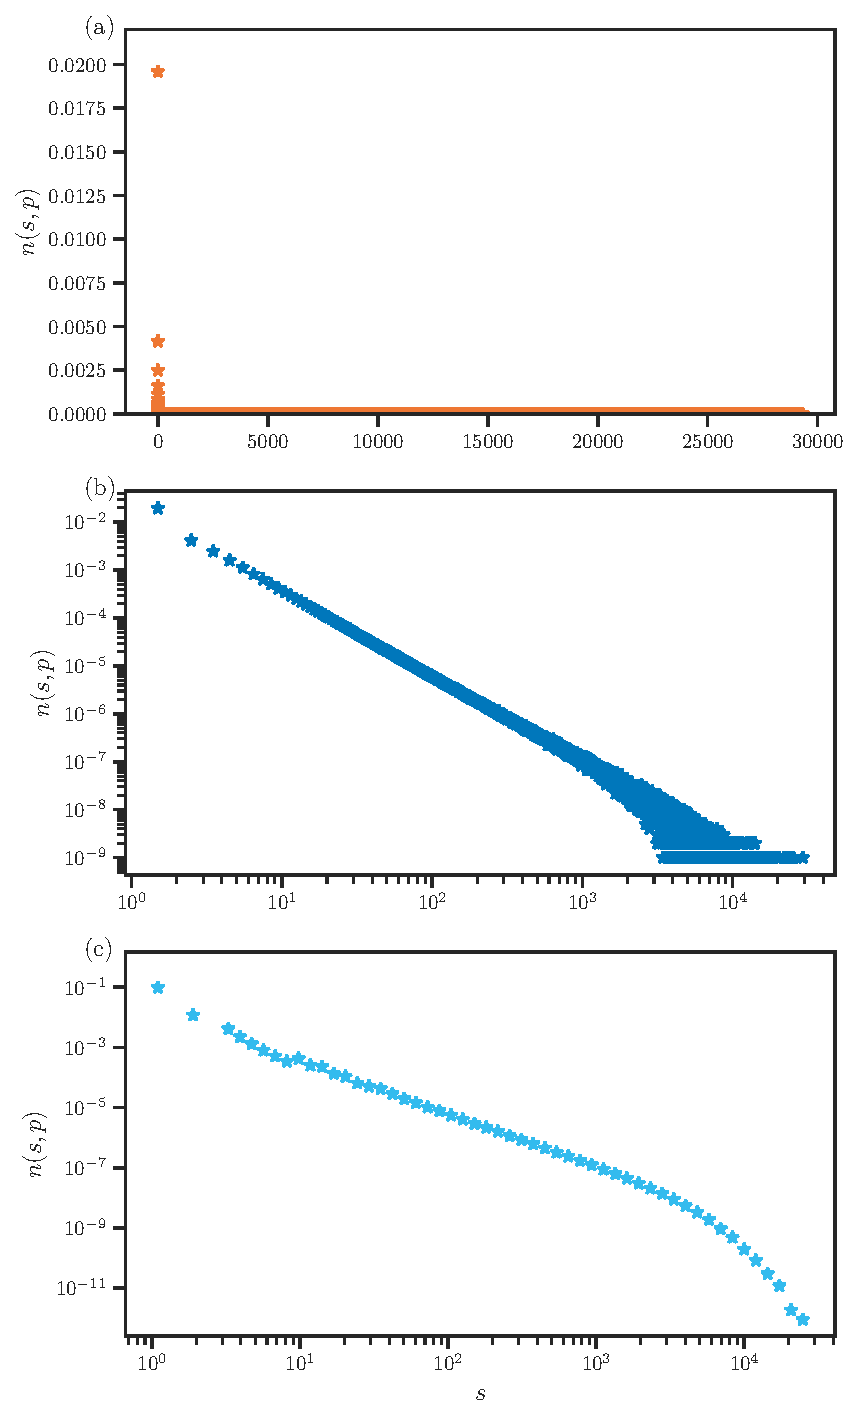
\includegraphics[width=\imsize]{num_clusteres_red_cuadrada.pdf}
	\caption[Gráfico de $n(s, p; L)$ estimado a partir de $M = 1000$ muestras para  $p=0.57$ y $L = 1000$.]{Gráfico de $n(s, p; L)$ estimado a partir de $M = 1000$ muestras para $p=0.57$ y $L = 1000$. (a) Gráfico directo. (b) Gráfico log-log. (c) Gráfico de la distribución agrupada logarítmicamente.}\label{f:num_clusteres_red_cuadrada}  
\end{figure}


\subsubsection{Mediciones de $n(s, p)$ cuando $p \to p_c$}\label{sec_critico}

¿Qué sucede con $n(s, p;L)$ cuando cambiamos $p$ para que se acerque a $p_c$? Realizamos una secuencia de simulaciones para varios valores de $p$ para la red anteriormente simulada y trazamos los valores resultantes para $\overline{n(s, p; L)}$. El gráfico resultante se muestra en la \Cref{f:num_cluster_critico}. Dado que el gráfico es doblemente logarítmico, una línea recta corresponde a un comportamiento de tipo ley de potencia, $n(s, p) \propto s^{-\tau}$.  En el caso de una red cuadrada bidimensional el valor del umbra critico es $p_c\approx0.592746$ (ver \Cref{table:umbral}), que en la  \Cref{f:num_cluster_critico} es la linea roja. Esto  sugiere que en este valor de $p$ el algoritmo que calcula la distribución de clústeres da un comportamiento que puede describirse mediante una ley de potencia, tal como se esperaba. Como se discutió en  el \cref{sec:leypotencia_intro}   el  hecho que un histograma de la ley de potencias presente una relación lineal en un gráfico doblemente logarítmico es una condición necesaria pero no suficiente para decir que los datos siguen una distribución de tipo ley de potencia. Por lo que la inspección visual de un diagrama puede generar falsos positivos.  Sumado a esto  ajustar con precisión una distribución de ley de potencia a datos empíricos, así como medir la bondad de ese ajuste, no es trivial. Para solventar estas dificultades aplicamos los métodos descritos en el \cref{sec:leypotencia} tanto para ajustar y evaluar distribuciones de colas pesadas en los datos. La implementación del algoritmo LSavg en Python se encuentra disponible en el repositorio de GitHub  de los autores \url{https://github.com/xszhong/LSavg/tree/main}.  


\begin{figure}[h!]
	\centering{}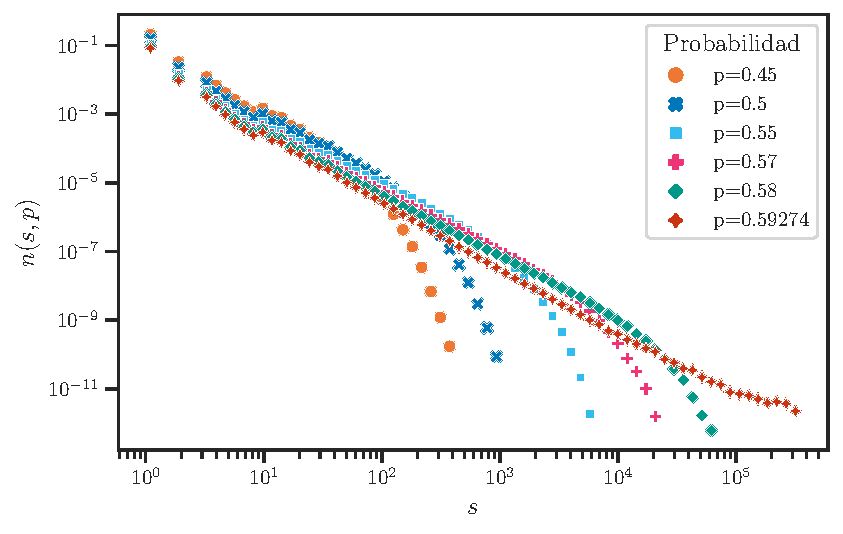
\includegraphics[width=\imsize]{num_cluster_critico.pdf}
	\caption[Gráfico de $n(s, p; L)$ en función de $s$ para varios valores de $p$ para una red de $1000\times1000$.]{Gráfico de $n(s, p; L)$ en función de $s$ para varios valores de $p$ para una red de $1000\times1000$.}\label{f:num_cluster_critico}  
\end{figure}



Para comprobar el funcionamiento del método de ajuste de leyes de potencia, se simularon $M=1000$ realizaciones  aleatorias de    una red cuadrada con  $L=1000$ y $p=p_c\approx0.592746$. Las estimaciones estadísticas de $n(s, p)$  
se agrupan mediante un conjunto de puntos de datos $\left\{\left(x_i,f(x_i)\right)\right\}$ en orden ascendente por sus valores $x$, donde $f(x_i)$ es la frecuencia de $x_i$ en la muestra. Ademas establecemos cuatro puntos de datos críticos cuyos valores de $x$ son $X_{5th}$ , $X_f$ , $X_1$ , $X_{max}$.  Por conveniencia, usamos los cuatro valores críticos de $x$ para representar sus puntos de datos correspondientes y los usamos con llaves para representar el subconjunto de puntos de datos desde el primer punto de datos hasta ellos; por ejemplo, $\{ X_{5th}\}$ representa el conjunto de los primeros cinco puntos de datos mientras que $\{ X_1 \}$ representa el conjunto de puntos de datos desde el primero hasta $X_1$. Las definiciones de estos puntos de datos críticos son las siguientes. $X_{5th}$ indica el quinto punto de datos. $X_f$ indica el último punto de datos en el que todos los puntos de datos de $\{ X_f \}$ satisfacen la propiedad  estrictamente decreciente del punto de datos ; mientras que su primer punto de datos posterior no satisface  esta  propiedad. $X_1=\min\left\{x_i\mid f(x_i)=\frac{1}{n}\right\}$ indica el primer punto de datos cuya frecuencia es $1/n$. $X_{max} = \max\left\{x_i\right\}$ indica el último punto de datos. Según las definiciones anteriores, la relación entre ellos es $X_f \leq  X_1 \leq X_{max}$.


Supongamos que el muestreo es perfecto (lo que significa que los datos muestreados siguen perfectamente una distribución de ley de potencia), la frecuencia del punto de datos de menor frecuencia es $1/n$ y sea este punto de datos $(X^T_1,1/n)$ entonces resolviendo $p(X^T_1)=K\cdot1/n$, obtenemos $X^T_1=(K\cdot n)^{1/\alpha}$. Esto significa que $X^T_1\propto n^{1/\alpha}$, y cuando $n \to\infty, X^T_1\to\infty$ \cite{zhong_is_2022}. Si el muestreo es perfecto, entonces $X_f=X_1=X^T_1=X_{max}$ según sus definiciones. Sin embargo, para una muestra de tamaño finito, el muestreo no es perfecto en la realidad y estos valores críticos no son iguales. Su relación empírica es $X_f<X_1<X^T_1\ll X_{max}$.



El resultado se muestra en la \Cref{f:ley_potencia_red_cuadrada}.  El \cref{table:valoresalpha_redcuadrada}  reporta el resultado de aplicar LSE para ajustar los datos discretos.  $\hat{\alpha}_{5th},  \hat{\alpha}_{f}, \hat{\alpha}_{X1}$ y $\hat{\alpha}_{all}$ indican el  $\hat{\alpha}$  ajustado por $LS_{norm}$ en $\{X5th\}, \{X_f\}, \{X_1\}$, y $\{X_{max}\}$, respectivamente. Mientras los que contienen el súper indice $avg$   indican el  $\alpha$ ajustado por $LS_{avg}$ en los puntos de datos correspondientes.   El \cref{table:valoresalpha_redcuadrada}   muestra  que  $\alpha_{all}$ tiene un valor de $0.7802$, lo que supone un sesgo significativo con respecto al valor real de $36/91$ reportado en la literatura (ver \Cref{table:exponentepercolacion} ).  Esta estimación sesgada es consistente con la reportada por los críticos de los métodos LSE. El mal resultado de este ajuste se debe a que se incluyen los ruidos de cola larga, los cuales no pueden tratarse como datos de ley de potencia.






\begin{figure}[h!]
	\centering{}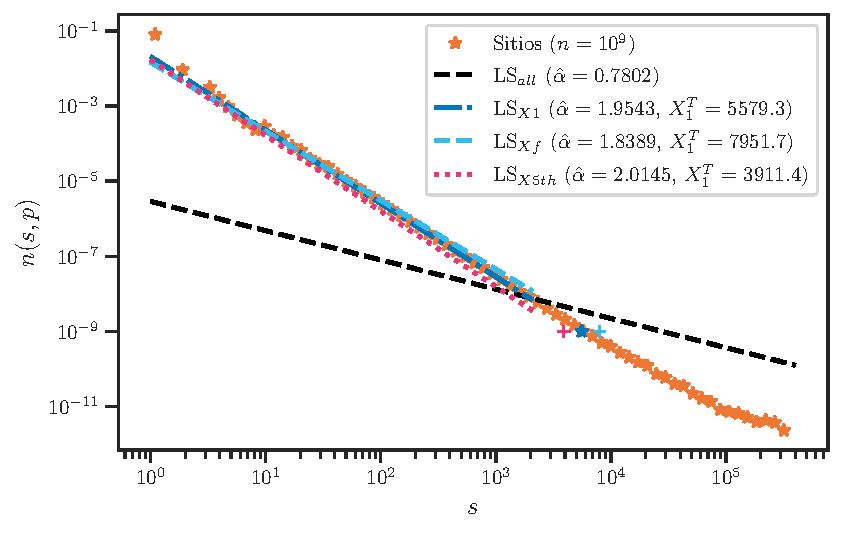
\includegraphics[width=\imsize]{ley_potencia_red_cuadrada.pdf}
	\caption[Métodos LSE  aplicados a la distribución de tamaños de clústeres $n(s,p$) para la red cuadrada para $L=1000$ y $M=1000$ realizaciones aleatorias.]{Métodos LSE  aplicados a la distribución de tamaños de clústeres $n(s,p$) para la red cuadrada para $L=1000$ y $M=1000$ realizaciones aleatorias. $LS_{all}$ indica la aplicación de $LS_{norm}$ a todos los datos para estimar $\alpha$. $LS_{X5th}$ indica la aplicación de $LS_{avg}$ a $\{X_{5th}\}$ para estimar $\alpha$; $LS_{Xf}$ aplica $LS_{avg}$ a $\{X_f\}$; y $LS_{X1}$ aplica $LS_{avg}$ a $\{X_1\}$. $X_1^T=\left(\hat{K}\cdot n\right)^{1/\hat{\alpha}}$ es el valor $x$ de  $(X^T_1,1/n)$ donde $n$ es el tamaño de la muestra.}\label{f:ley_potencia_red_cuadrada}  
\end{figure}




	


\begin{table}[h!]
	\centering
	\caption[Estimación de $\alpha$ para el ajuste de  la distribución de tamaños de clústeres $n(s,p$) para la red cuadrada para $L=1000$ y $M=1000$ realizaciones aleatorias.]{Estimación de $\alpha$ para el ajuste de  la distribución de tamaños de clústeres $n(s,p$) para la red cuadrada para $L=1000$ y $M=1000$ realizaciones aleatorias.}
	\begin{tblr}{colspec={lllllll},
			row{odd} = {bg=gray8},
			row{even} = {bg=gray9},
			row{1} = {bg=red3, fg=white, font=\sffamily},
		}
		
		$\hat{\alpha}_{5th}$ &  $\hat{\alpha}_{5th}^{avg}$ & $\hat{\alpha}_{f}$  & $\hat{\alpha}_{f}^{avg}$  & $\hat{\alpha}_{X1}$ &  $\hat{\alpha}_{X1}^{avg}$ &  $\hat{\alpha}_{all}$ \\
		
		{2.0145} &  {2.01446} & {1.8389} & {1.8388} & {1.9543} & {1.9542} & {0.7802}
		
	\end{tblr}
	\label{table:valoresalpha_redcuadrada}
\end{table}



\begin{table}[h!]
	\centering
	\caption[Estimaciones para los exponentes críticos de la teoría de percolación de varios sistemas. ]{Estimaciones para los exponentes críticos de la teoría de percolación de varios sistemas}
	\begin{tblr}{colspec={lllllllllll},
			row{odd} = {bg=gray8},
			row{even} = {bg=gray9},
			row{1} = {bg=red3, fg=white, font=\sffamily},
		}
		
		dimensión & $\beta$ & $\tau$ & $\sigma$ & $\gamma$ & $\nu$ & $D$ & $\mu$ & $D_{min}$ & $D_{max}$ & $D_B$ \\
		1 &  & 2 & 1 & 1 & 1 & &&&&&\\
		2 & 5/36 & 	187/91 & 36/91 & 43/18 & 	4/3 &	91/48 & 1.30 &	1.13 & 	1.4 & 1.6 \\
		3 & 0.41 &	2.18 & 	0.45 & 	1.80 & 	0.88 & 	2.53 & 	2.0 & 	1.34 & 	1.6 & 	1.7 \\
		4  & 0.64 & 2.31 & 	0.48 & 	1.44 & 	0.68 & 	3.06 & 	2.4 & 	1.5 & 	1.7 & 	1.9		\\
		Bethe & 	1 & 5/2 & 	1/2 & 	1 & 	1/2 & 	4 & 	3 & 	2 & 	2 & 2
	\end{tblr}
	\label{table:exponentepercolacion}
\end{table}

	Tanto $\hat{\alpha}_{5th}$,  $\hat{\alpha}_{5th}^{avg}$, $\hat{\alpha}_{f}$, $\hat{\alpha}_{f}^{avg}$, $\hat{\alpha}_{X1}$ y   $\hat{\alpha}_{X1}^{avg}$ se estiman sin  los ruidos de cola larga. Todos ellos oscilan alrededor del valor verdadero de $\alpha$.  Específicamente $\hat{\alpha}_{5th}^{avg}=2.014$ se acerca mucho más al valor verdadero.  Esto significa que, al excluir los ruidos de cola larga, $\hat{\alpha}$ cambia de significativamente sesgado a casi no sesgado. Son los ruidos de cola larga los que causan un sesgo significativo en el LSE.  Comparando los $\hat{\alpha}$ con los $\hat{\alpha}^{avg}$, podemos ver que $LS_{avg}$ funciona mucho mejor que  $LS_{norm}$.  La razón es que la estrategia de promediado utilizada en $LS_{avg}$ reduce el impacto de aquellos puntos de datos desviados de la línea de regresión. La  \Cref{f:ley_potencia_red_cuadrada}  demuestra que $LS_{avg}$ se ajusta perfectamente a los datos de la ley potencial.
	
	
	
Después de obtener los modelos de ley de potencia estimados, calculamos sus estadísticas KS correspondientes en $\{ X_1 \}$, escogemos $D_n^{X_{5th}}$ por tener el valor  mínimo de $D_n$.  Del modelo de ley de potencia estimado extraemos 500 muestras, luego calculamos $D_n^T$ por la  \Cref{eq:98} (ver \Cref{table:valoresD_redcuadrada})  y utilizamos la estrategia descrita en el \cref{procedimiento1}. En este conjunto de datos $D_n^T=0.086$ y $D_n^{X_{5th}}=0.067$ por lo que se cumple que $D_n\leq D_n^T$ entonces aceptamos la hipótesis $H_0$ de que los datos son sacados de una distribución de tipo de ley de potencia, lo que era de esperar ya que se sabe que estos datos siguen esta distribución. Lo anterior evidencia que el algoritmo esta funcionando correctamente y puede  utilizarse para ayudarnos a corroborar la hipótesis de  que los clústeres de neuronas  en los experimentos de C. elegans  siguen una ley de potencias evidenciando  un comportamiento critico. 


 \begin{table}[h!]
	\centering
	\caption[Valores máximos de $D_{n,n}$  y sus p-valores de la prueba KS de muestras extraídas del modelo de ley de potencias con $\alpha = 2.015$ y $n = 10^4$. ]{ Valores máximos de $D_{n,n}$  y sus p-valores de la prueba KS de muestras extraídas del modelo de ley de potencias con $\alpha = 2.015$ y $n = 10^4$.  El tamaño indica el número de muestras en el grupo.}
	\begin{tblr}{colspec={lll},
			row{odd} = {bg=gray8},
			row{even} = {bg=gray9},
			row{1} = {bg=red3, fg=white, font=\sffamily},
		}
		
			Tamaño & $D_{n,m}$  &  $p_{value}$  \\
             100        &  {0.069} & {0.01709} \\
             200        & {0.086}  & {0.0012} \\
             300        & {0.086}  & {0.00122} \\
             400        & {0.094}  & {0.00028} \\
             500        & {0.094} & {0.00028} \\
	\end{tblr}
	\label{table:valoresD_redcuadrada}
\end{table}

\subsection{Estadísticas de los clústeres de la actividad neuronal }\label{eq:estadistica_cllusteres}


En la parte  anterior se utilizo un modelo de control para corroborar el funcionamiento del algoritmo del calculo de clústeres y del ajustes de colas pesadas. En esta parte se estudiara los patrones de actividad espacio-temporal que emergen de la dinámica cerebral completa de los experimentos de C elegans siguiendo los métodos anteriormente descritos.  La actividad cerebral completa se caracterizó por la activación de grupos de neuronas que podían abarcar grandes partes del cerebro. Nuestro objetivo es describir las estadísticas de estos eventos.  Para ello, la actividad de cada  neurona se binarizó utilizando los métodos descritos en los \cref{sec:umbralizacion,sec:inferencia_spikes}. Para los 21 gusanos de los experimentos de Yemini et al \cite{yemini_neuropal_2021} se utilizo el método de Kaplan de inferencia de picos en la traza  $\Delta F/F$ de cada conjunto de datos. Por otro lado, en el resto de experimentos (Kato et al \cite{kato_global_2015}, Kaplan et al \cite{kaplan_nested_2020})  se utilizo el método CASCADE para la inferencia de spikes con un umbral adecuado . A continuación, identificamos grupos de neuronas coactivadas y espacialmente contiguas y cuantificamos su número, tamaño y evolución en el tiempo.


Para caracterizar los grupos de neuronas coactivadas y espacialmente contiguas se utilizó  un enfoque de modelado híbrido que combina el conectoma del C. elegans hermafrodita reconstruido por Cook et al.  \cite{cook_whole-animal_2019}  junto con   los registros   de  las  series temporales de la dinámica neuronal binarizada  de los tres experimentos   con C. elgans. Las conexiones sinápticas entre pares de neuronas en todo el sistema nervioso (connectoma) se han descrito completamente.  Una desventaja de este método, es que  solo consideramos las neuronas etiquetadas, por lo que la cantidad de series temporales usadas para los cálculos puede ser menor que la serie neuronal Completa.  En cada paso de tiempo  se agrupan los spikes de neuronas  que comparten el mismo tipo de actividad conectados siguiendo la matriz de adyacencia del conectoma de Cook y posteriormente mediante el algoritmo descrito en el \cref{sec:alg_cluster} se calcula el tamaño del clúster, el cual  es el número total de neuronas participantes.  Posteriormente para cada tiempo $t$, calculamos la proporción de neuronas activas ($\left\langle A(t) \right\rangle$), el número de clústeres ($m$) y el tamaño del $i$-ésimo clúster ($C_s(i), 1 \leq i \leq m$ ).  



En primer lugar, tal como se realizo en  \cite{ponce-alvarez_whole-brain_2018,tagliazucchi_criticality_2012} calculamos la relación entre $\left\langle A(t) \right\rangle$ y $m$ encontrando  que  siguen una relación no lineal que se asemeja a la de la percolación.  El número de clústeres alcanzaba su máximo en un nivel crítico de actividad global  $ \left\langle A(t) \right\rangle \approx 11\%$ para los experimentos de Yemini et al \cite{yemini_neuropal_2021},  un valor que denotamos como $\left\langle A(t) \right\rangle_c$ (línea  vertical discontinua rosada en la  \Cref{fig:estadisticas_clusteres_neuropal}(a)). La variabilidad de $m$ también se maximizaba a este nivel de activación.  Ademas La correlación entre el la densidad  de sitios activos (un índice de la actividad total) y el número de clústeres se invierte por encima de este umbral crítico de actividad, una característica que ya se ha descrito en otros sistemas complejos en los que alguna densidad creciente compite con la capacidad limitada. Este resultado es interesante porque sugiere que la actividad neuronal colectiva se organiza de forma más compleja en un rango intermedio de actividad neuronal. A bajos niveles de actividad, hay pocos clústeres y la actividad neuronal está muy dispersa. A altos niveles de actividad, hay un gran clúster dominante y la actividad neuronal es más homogénea. Sin embargo, a niveles de actividad intermedios, hay una mayor diversidad de clústeres, lo que sugiere que la actividad neuronal está más organizada y que hay una mayor interacción entre diferentes grupos de neuronas. Con respecto a la variabilidad existe una mayor incertidumbre en el número de clústeres que se observarán en $\left\langle A(t) \right\rangle_c$. Esto podría deberse a que el sistema está en un punto crítico en el que pequeños cambios en la actividad neuronal pueden conducir a grandes cambios en la organización de la actividad neuronal colectiva.

\begin{figure}[h!]
	\centering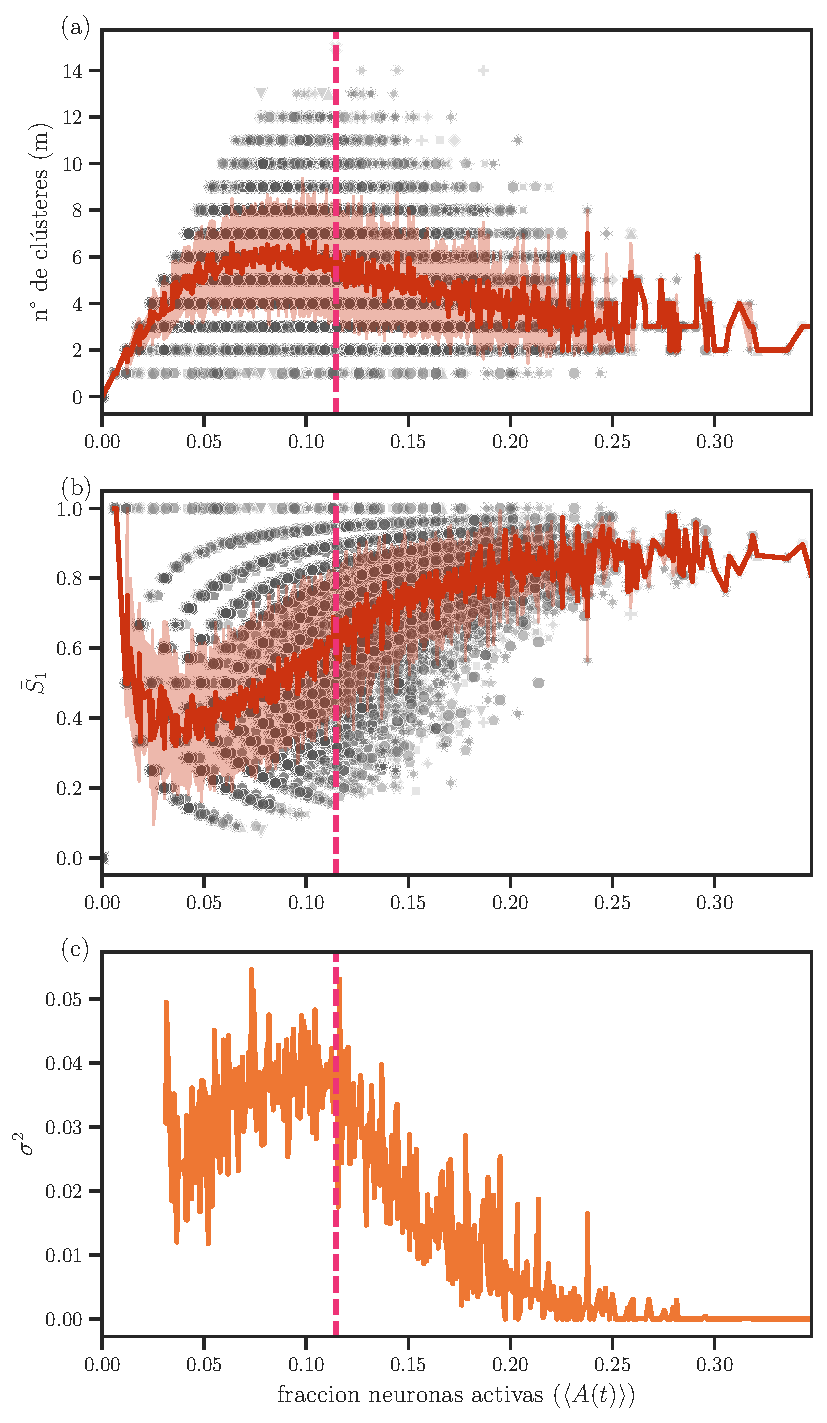
\includegraphics[width=\imsize]{estadisticas_clusteres_neuropal.pdf}
	\caption[ El nivel de actividad cerebral fluctúa continuamente por encima y por debajo de una transición de fase.] {El nivel de actividad cerebral fluctúa continuamente por encima y por debajo de una transición de fase.  (a) Número de clústeres ($m$) en función de la proporción de neuronas activas ($\left\langle A(t) \right\rangle$) para los distintos grupos de datos de los experimentos con C. elegans  de Yemini et al. Cada punto de diferente intensidad de gris  y forma es un gusano distinto. Línea roja, es la media de $m$; área roja, su desviación estándar.  (b)   El parámetro de orden, definido aquí como el tamaño (normalizado) del clúster más grande, se representa en función de la fracción de sitios activos $\left\langle A(t) \right\rangle$ ( los promedios se representan con la curva roja).   (c) La varianza del parámetro de orden ($\sigma$) aumenta como se espera para una transición de fase. Ademas se observa que el pico de $\sigma$ en este panel coincide con el pico del número de clusteres $m$  en  (a). } \label{fig:estadisticas_clusteres_neuropal}
\end{figure}


Las anteriores  características recuerdan a otros sistemas complejos que atraviesan una transición de fase orden-desorden
por lo que siguiendo técnicas estándar de la  física estadística, se definieron y calcularon dos parámetros a partir de los parametros $C_s$ y $\left\langle A(t) \right\rangle$.  Para representar el grado de orden (es decir, el parámetro de orden), se calculó el tamaño normalizado del clúster más grande (es decir, $\bar{S}_1 = \max(C_s)/N_{E}$, donde $N_E$  es el número de sitios activos) en todo el cerebro y se representó en función del número de puntos activos (es decir, el parámetro de control).  Esto se hizo para todos los pasos de tiempo de los 21 gusanos. La \Cref{fig:estadisticas_clusteres_neuropal}(b) muestra la relación entre $\left\langle A(t) \right\rangle$ y el tamaño normalizado del clúster más grande.  Encontramos  varias características clave, todas muy sugestivas de una transición de fase.  En primer lugar, hay un fuerte aumento en el parámetro de orden promedio (linea roja), acompañado de un aumento de su variabilidad (\Cref{fig:estadisticas_clusteres_neuropal}(c)). En segundo lugar, la transición coincide con el pico en la función discutida en la Figura \Cref{fig:estadisticas_clusteres_neuropal}(a), que representa el número (no el tamaño) de los clústeres.  Finalmente encontramos que $\bar{S}_1$ crece con $\left\langle A(t) \right\rangle$  y abarca un amplio rango de escalas, desde unas pocas neuronas hasta una gran proporción del cerebro  lo que indica que la mayor parte de las neuronas están coactivadas.     Por lo tanto, el hecho de que el clúster más grande abarque una gran parte del cerebro también podría ser un indicador de criticidad neuronal.


Se encontró también  la distribución de $\left\langle A(t) \right\rangle$ , denotada como $p(\left\langle A(t) \right\rangle)$ utilizando el histograma de los datos de Yemini et al y su KDE. En la mayoría de los casos, el nivel de activación espontánea estaba por debajo de $\left\langle A(t) \right\rangle_c$, y entre el 10\% y el 30\% del tiempo,  $p(\left\langle A(t) \right\rangle)$ era mayor que  $p(\left\langle A(t) \right\rangle)_c$ (\Cref{fig:distactivos}). 



\begin{figure}[h!]
	\centering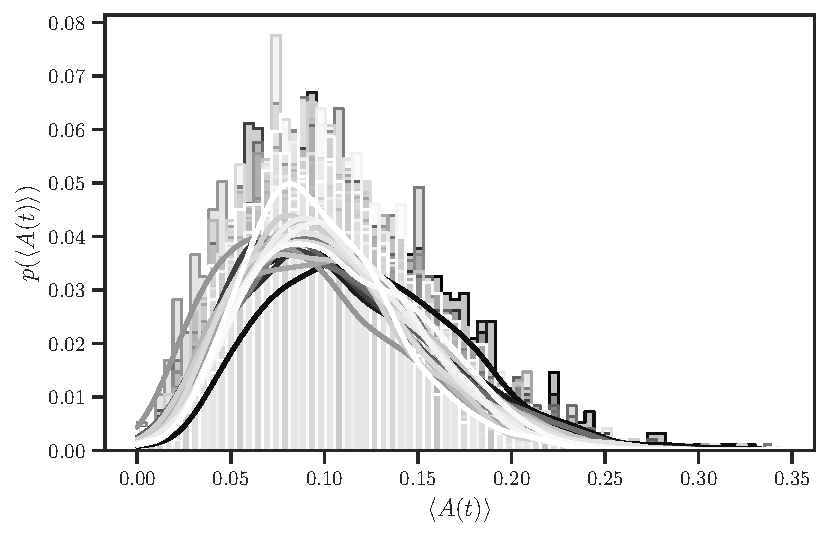
\includegraphics[width=\imsize]{distactivos.pdf}
	\caption[Distribución de $p(\left\langle A(t) \right\rangle)$    calculada para cada uno de los  21 gusanos del conjunto de datos de Yemini et al.]{Distribución de $p(\left\langle A(t) \right\rangle)$    calculada para cada uno de los  21 gusanos del conjunto de datos de Yemini et al. Se calculo también la KDE de cada distribución.} \label{fig:distactivos}
\end{figure}

Finalmente para identificar si los  grupos de neuronas que pertenecen a un mismo clúster presentan  un patrón de actividad similar y  poder cuantificar su sincronía, utilizamos un enfoque basado en la correlación cruzada con retardo en ventana deslizante  (RWTLCC).  Este proceso realiza una correlación cruzada con retardo en múltiples ventanas de la señal. El resultado es una serie temporal de correlaciones cruzadas, que muestra cómo la interacción entre las dos señales cambia a lo largo del tiempo. 

Para realizar este calculo,  en un determinado paso de tiempo   se seleccionaron  al azar dos pares de neuronas pertenecientes al mismo clúster $s$  del conjunto de datos del gusano 1 de Kaplan et al y otro par que no pertenecían al mismo clúster.   Posteriormente  a este par de neuronas se le realizaron  dos  pruebas de dependencias estadísticas en su actividad de calcio. En primer lugar, se realizo una  inspección visual de su sincronización y posteriormente se   calculó el correlograma mediante  RWTLCC del trazo de fluorescencia. Cuando las neuronas pertenecen al mismo clúster (señales azules y naranjas en la \Cref{fig:correlaciones_clusteres})  tanto la inspección visual como el correlograma muestran una similitud temporal entre estos dos  pares de neuronas. Por el contrario si no hacen parte del mismo clúster (señales verdes y rosadas)  no  existe esta similitud. Nótese como el correlograma no muestra sincronización en este ultimo caso. 


\begin{figure}[h!]
	\centering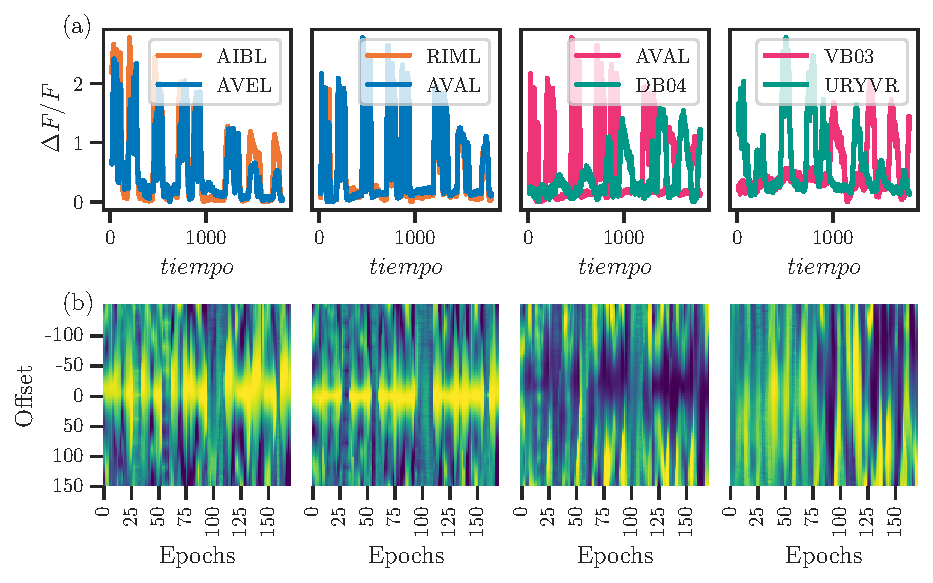
\includegraphics[width=\imsize]{correlaciones_clusteres.pdf}
	\caption[Prueba de dependencias estadísticas en la actividad de calcio de dos pares de neuronas que pueden hacer parte o no de un mismo clúster.]{Prueba de dependencias estadísticas en la actividad de calcio de dos pares de neuronas que pueden hacer parte o no de un mismo clúster.   (a)  inspección visual de sincronización entre las dos neuronas (b)   correlograma del algoritmo  RWTLCC aplicado a la  traza de fluorescencia.  Las señales azul y naranja pertenecen a un mismo clúster mientras que las señales verde y rosado no hacen parte del mismo clúster.  } \label{fig:correlaciones_clusteres}
\end{figure}





\subsection{Distribución del tamaño de clústeres $n(s,p)$}\label{sec:distribucion_tamaño}


Los comportamientos anteriores son firmas de la existencia de un punto crítico de percolación ($p_c$). La teoría de la percolación muestra que, cerca de la probabilidad crítica, la distribución de los tamaños de los clústeres sigue una ley de potencias con un exponente que solo depende de las dimensiones del sistema (no depende de los detalles del sistema físico). Para probar esto, calculamos la distribución de los tamaños de los clústeres $P(n(s,p))$ en cada conjunto de datos y la aproximamos por una ley de potencias, que aparece como una línea recta en una gráfica log-log con binneo logarítmico, de modo que $P(n(s,p)) \sim s^{-\tau}$ (\Cref{fig:ley_potencia_experimentos}).


\begin{figure}[h!]
	\centering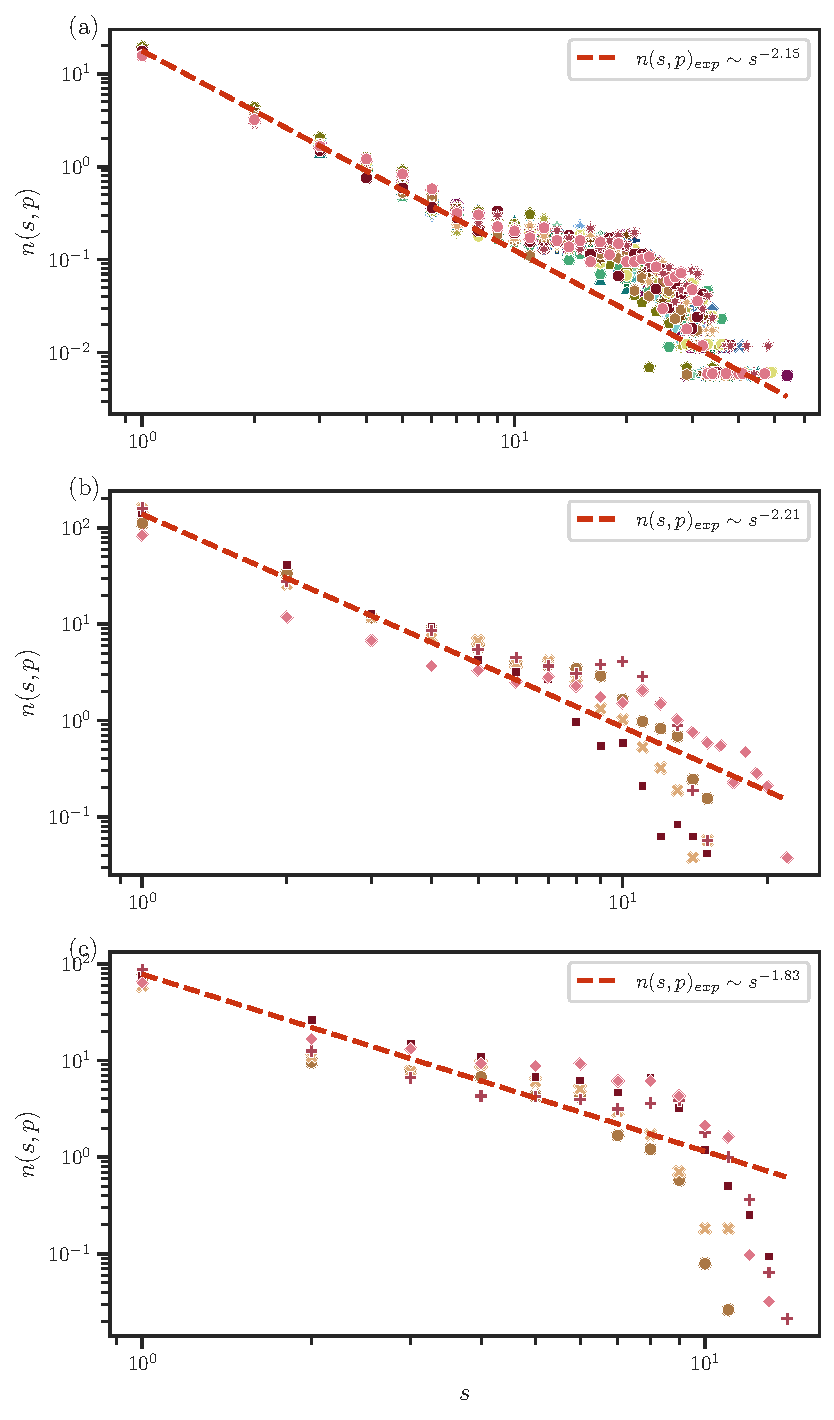
\includegraphics[width=\imsize]{ley_potencia_experimentos.pdf}
	\caption[Distribución de tamaños de los clústeres $n(s,p)$ para los conjuntos de datos de los distintos experimentos con C. elgans: (a) Yemini et al. (b) Kaplan et al. (c) Kato. et al. ]{Distribución de tamaños de los clústeres $n(s,p)$ para los conjuntos de datos de los distintos experimentos con C. elgans: (a) Yemini et al. (b) Kaplan et al. (c) Kato. et al. Cada punto con diferente color y forma es un gusano correspondiente a cada conjunto de datos.  La linea roja  es el mejor ajuste de la ley de potencia a la distribución de tamaños de clústeres. } \label{fig:ley_potencia_experimentos}
\end{figure}

Aplicamos los métodos LSavg y MLE discutidos en el \Cref{sec:leypotencia} para ajustar las distribuciones de ley de potencia de los conjuntos de datos. Como se discutió anteriormente el algoritmo de LSavg se encuentra en el repositorio de GitHub de los autores \footnote{\url{https://github.com/xszhong/LSavg}}.  Para la implementación de MLE utilizamos la caja de herramientas NCC (Neural Criticality and Complexity) de  Matlab \cite{marshall_analysis_2016}  que se encuentra disponible en \url{http://www.nicholastimme.com/software.html}.  En el caso del algoritmo de LSavg  para cada conjunto de puntos de datos,  aplicamos LSavg en  $X_{5th}$, $X_f$ y $X_1$ ( para una discusión de estos valores ver el \Cref{sec_critico})   y denotamos el $\tau$ inferido por $\tau(X_{5th}), \tau(X_f)$ y $\tau(X_1)$. Estos tres puntos de datos críticos se utilizan para definir el rango de ajuste de la ley de potencia truncada.  Después de obtener los modelos de ley de potencia estimados, calculamos sus estadísticas KS correspondientes $D_n$, y elegimos  el mínimo y su modelo correspondiente como resultados finales de este método. En este caso el conjunto $X_{5th}$ es el que tiene mejores resultados. 

 La \cref{fig:exponentes_experimentos}   muestra los $\tau$ ajustados por LSavg en los puntos de datos que dieron el mejor resultado ($X_{5th}$).   El exponente de la ley de potencia correspondiente $\tau$ estaba entre $1.8$ y $2.22$ para los diferentes conjuntos de datos, con unos promedios de $2.1478\pm 0.06$, $2.2104\pm0.24$, $2.022\pm0.356$ para los experimentos de Yemini et al, Kaplan et al y Kato et al respectivamente. El mejor resultado (menor desviación estándar) se obtuvo con el conjunto de datos de Yemini et al. Este resultado  era esperable debido al hecho que este conjunto tiene etiquetadas aproximadamente 170 neuronas en cada gusano, comparado con las 50 y 39 neuronas etiquetadas en los conjuntos de Kaplan et al y Kato et al.  Dado que nuestro método requiere encontrar los vecinos de las neuronas utilizando la matriz de adyacencia del conectoma de C. elegans, el numero de neuronas conocidas es importante. El bajo numero de neuronas etiquetadas en los experimentos de Kaplan et al y Kato et al  se debe a las clásicas  limitaciones del registro neuronal por el método de imágenes de Calcio.  Por otro lado, los gusanos transgénico desarrollados por Yemini et al conocidos como  Neuropal fueron diseñados con el objetivo de superar estas falencias, de ahí que todo el set de datos tiene la totalidad de sus neuronas etiquetadas. 
 
  


 \begin{figure}[h!]
 	\centering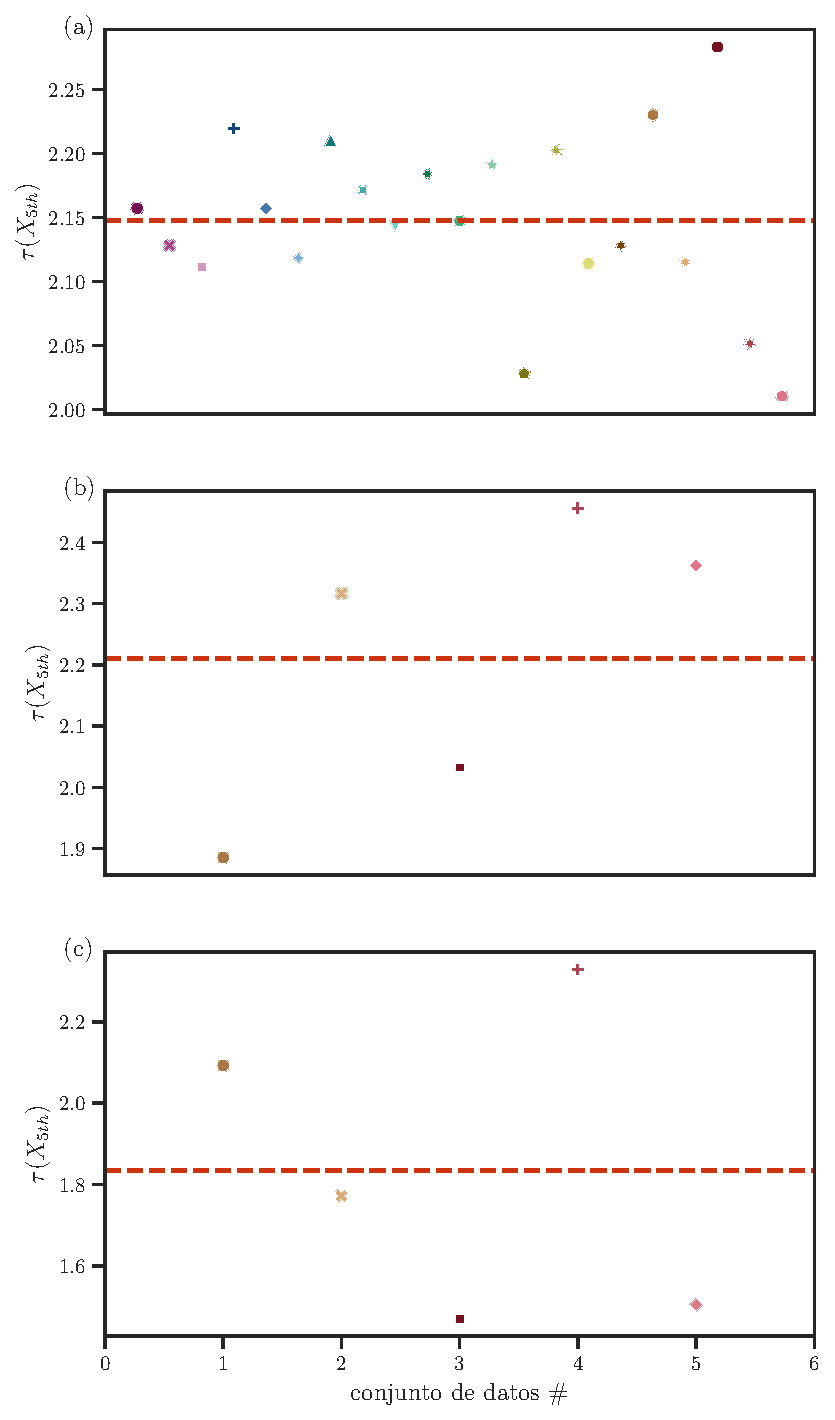
\includegraphics[width=\imsize]{exponentes_experimentos.pdf}
 	\caption[ Exponentes de potencia $\tau$ estimados usando LSavg en los distintos conjuntos de datos. (a) Yemini et al. (b) Kaplan et al. (c) Kato et al. Cada punto es un gusano diferente. ]{ Exponentes de potencia $\tau$ estimados usando LSavg en los distintos conjuntos de datos. (a) Yemini et al. (b) Kaplan et al. (c) Kato et al. Cada punto es un gusano diferente. La linea roja punteada se corresponde al valor de $\tau$ promedio en todos los gusanos de un mismo experimento. } \label{fig:exponentes_experimentos}
 \end{figure}
 
 
 Para corroborar los exponentes $\tau$ calculados anteriormente mediante el método LSavg en el conjunto de datos que dio el mejor resultado (Yemini et al), se procede a estimar la ley de potencia truncada que mejor se ajusta a la distribución   de estos datos  mediante  el algoritmo  de máxima verosimilitud (MLE).  El $\tau$ promedio (\Cref{fig:exponentes_experimentos2}(a)) tiene un valor de $\left\langle \tau \right\rangle =\approx 1.906 $  que es muy cercano al calculado con el otro método.   Los puntos  de truncamiento mínimo  y máximo   tienen un valor  promedio de $x_{min}=1$ y $x_max=15$ respectivamente.  Obsérvese que, el punto de truncamiento máximo coincide aproximadamente con el valor critico $\left\langle A(t) \right\rangle_c$, donde el numero de clústeres $m$ es máximo (\Cref{fig:mvsfrac}(a)).    
 
Para cuantificar si el ajuste de ley de potencia es aceptable, utilizamos el  algoritmo  descrito en el \cref{sec:ajusteybondad}.  Al aplicar este algoritmo en los distintos gusanos ( \cref{fig:exponentes_experimentos2}) encontramos un valor promedio de $p=0.2696\pm 0.05 \geq pthresh =0.2$, por lo que aceptamos que los datos se ajustan moderadamente (debido a su cercanía al valor de umbral) a la ley de potencia truncada porque las fluctuaciones de los datos reales de la ley de potencia fueron similares en el sentido de KS a las fluctuaciones aleatorias en un modelo de ley de potencia perfecto.  Tenga en cuenta que este método no puede probar que los datos se generaron mediante una ley de potencia truncada, sino que solo puede rechazar la hipótesis de la ley de potencia truncada. Dado al reducido tamaño del sistema podemos sugerir solamente que los datos pareciera seguir una ley de potencias. 
 

 
  \begin{figure}[h!]
 	\centering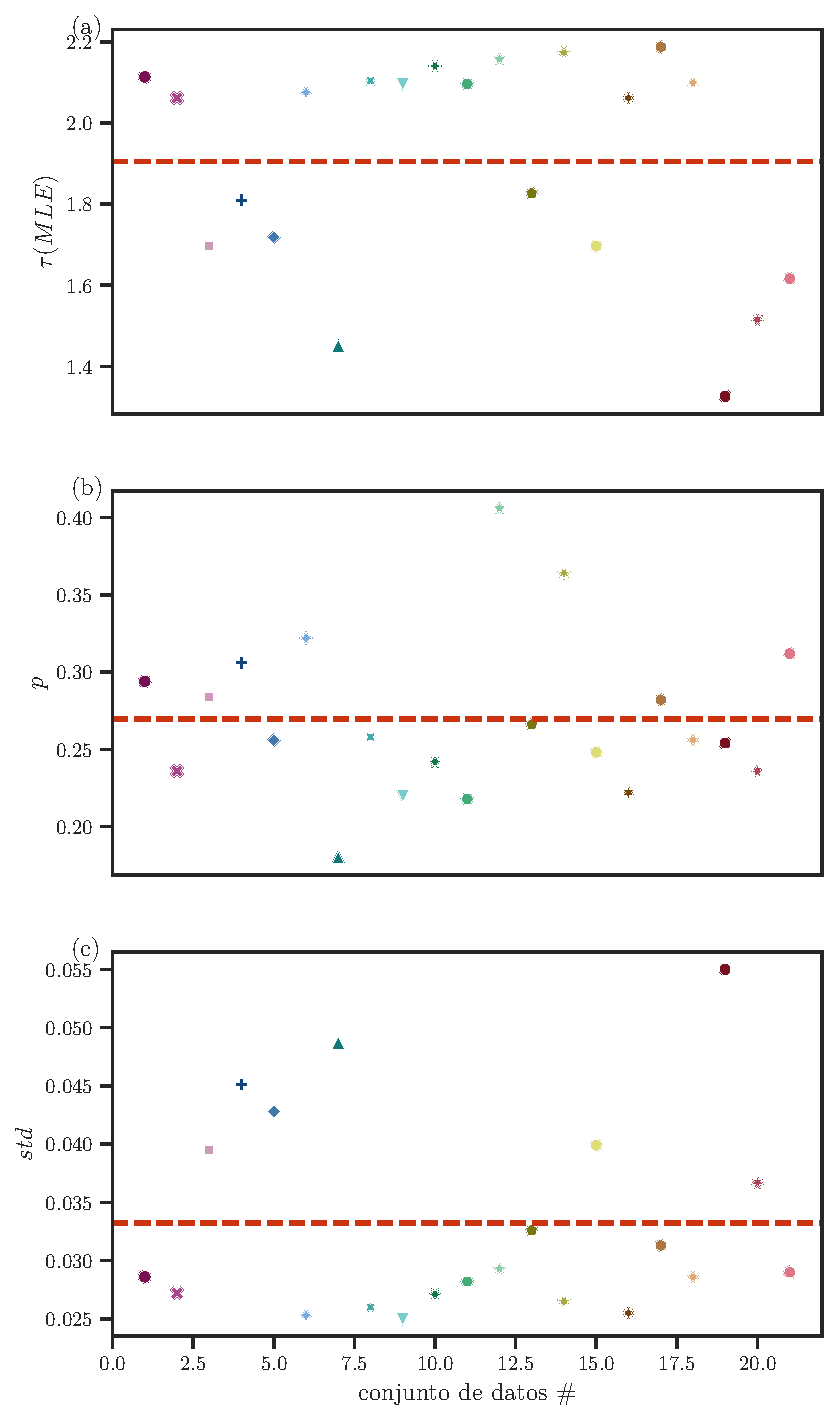
\includegraphics[width=\imsize]{exponentes_experimentos2.pdf}
 	\caption[ Estadísticas del ajuste  de máxima verosimilitud (MLE) en los distintos gusanos del  experimento  Yemini et al. ]{ Estadísticas del ajuste  de máxima verosimilitud (MLE) en los distintos gusanos del  experimento  Yemini et al. Cada punto es un gusano diferente. (a) Exponentes de potencia $\tau$ estimados usando un ajuste de máxima verosimilitud (MLE). La linea roja punteada se corresponde al valor de $\tau$ promediado en todos los gusanos. (b) Valores de $p$ para  para cuantificar  que tan bien es el ajuste en cada conjunto de datos. La linea roja punteada se corresponde al valor de $p$ promediado en todos los gusanos. (c) desviación estándar de los exponentes de la ley de potencia calculados mediante el algoritmo MLE. La linea roja punteada se corresponde al valor de la desviación estándar  promediada en todos los gusanos. } \label{fig:exponentes_experimentos2}
 \end{figure}
 
 
 
 
 \subsection{Longitud de correlación}
 
Como se abordo en el \Cref{sec:Sucebtibilidad}  longitud de correlación es una medida importante de la estructura de un sistema. Se puede utilizar para estudiar cómo se propaga la información o la energía a través de un sistema.  Podemos medir el tamaño típico de un clúster a partir de la función de correlación. La función de correlación $g(r, p)$, que es la probabilidad de que dos nodos, que están a una distancia $r$ entre sí, estén conectados y formen parte del mismo clúster para un sistema con probabilidad de ocupación $p$. Podemos utilizarla para definir la distancia cuadrática media entre dos sitios $i$ y $j$ que pertenecen al mismo clúster mediante la \Cref{eq:17}.  Para medir la función de correlación, utilizamos un algoritmo que recorre todos los pares de nodos en el sistema y calcula su distancia $r_{ij}$ mediante una métrica adecuada (camino mas corto, euclidiana, etc.).  Estimamos la probabilidad de que dos sitios a una distancia $r_{ij}$ estén conectados contando cuántos de los sitios que están a una distancia $r_{ij}$ están conectados, en comparación con cuántos sitios en total están a una distancia $r_{ij}$.  La distancia que utilizaremos en nuestros experimentos es la correspondiente al resolver el  problema del camino más corto que consiste  en encontrar un camino entre dos neuronas(nodos) del conectoma, de tal manera que la suma de los pesos de las aristas que lo constituyen sea mínima. Para realizar el calculo de esta longitud utilizamos la función de Scipy \textbf{csgraph.shortest\_path} \footnote{\url{https://docs.scipy.org/doc/scipy/reference/generated/scipy.sparse.csgraph.shortest_path.html}}, cuya entrada es el conectoma del C. elegans. 
 
 Al aplicar el algoritmo que calcula $g(r,p)$ junto con la distancia del camino mas corto a los datos experimentales obtenemos la \Cref{fig:correlacion_experimento}.   Encontramos la presencia de correlaciones funcionales de largo alcance entre las neuronas.   Las correlaciones  de largo alcance son un sello distintivo de los sistemas complejos en criticidad, que se caracterizan por dinámicas espaciotemporales colectivas emergentes no triviales.
 
   \begin{figure}[h!]
 	\centering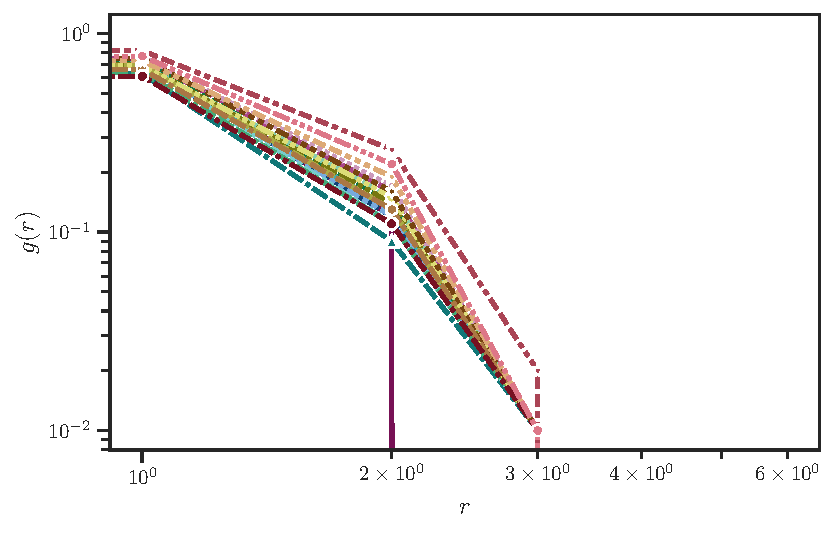
\includegraphics[width=\imsize]{correlacion_experimento.pdf}
 	\caption[  Función de correlación $g(r)$: correlación media entre pares de células en función de la distancia mas corta  $r$, para cada conjunto de datos de Yemini et al.]{  Función de correlación $g(r)$: correlación media entre pares de células en función de la distancia mas corta  $r$, para cada conjunto de datos de Yemini et al.} \label{fig:correlacion_experimento}
 \end{figure}

 
 
% 
%\section{Discusión}
%
%La reducción de la señal fMRI BOLD a eventos discretos no solo permite la identificación de redes de estado de reposo bien descritas como se muestra en la Figura 2, sino que también revela que la actividad cerebral a gran escala se organiza en avalanchas de actividad con distribuciones de tamaño de ley de potencias. El enfoque del proceso puntual permitió por primera vez identificar explícitamente los parámetros de orden y control y definir el estado del cerebro en reposo como una fluctuación alrededor de una transición de fase. El análisis muestra no solo que la actividad se propaga como avalanchas sin escala que se asemejan a las observadas en escalas más pequeñas (Beggs y Plenz, 2003)
%
%La observación de que la dinámica cerebral a gran escala puede rastrearse como avalanchas discretas sin escala de actividad plantea la cuestión de la relevancia fisiológica codificada en el momento de estos eventos a gran escala, ya sugerida por observaciones a escalas más pequeñas y modelos computacionales (Kinouchi y Copelli, 2006; Shew et al., 2009, 2011; de Arcangelis y Herrmann, 2010). Por ejemplo, aunque son relativamente raras, las avalanchas en la cola de la distribución de la ley de potencias surgen de un origen local y se propagan hasta la longitud de toda la corteza, lo que sugiere un papel en los procesos de vinculación de regiones corticales distantes. Sería interesante investigar si la interrupción total o parcial de estos grandes eventos, así como las alteraciones en el equilibrio entre activación y segregación en grupos, se correlacionan con condiciones patológicas y con el nivel de conciencia del sujeto.
%
%
%Además, la relación no lineal entre el tejido cortical activado y el número de grupos exhibe un punto óptimo, en el que el nivel de actividad cerebral se segrega en el número máximo de activaciones espacialmente aisladas. Podemos hipotetizar que este resultado es relevante para la solución del dilema integración/segregación propuesto por Tononi et al. (1994); Sporns (2010) como el enigma fundamental que la corteza sana necesita estar ejecutando en cualquier momento dado. Si nuestra hipótesis es verdadera, podemos predecir, junto con las teorías de integración/segregación de la conciencia (Tononi et al., 1994; Tononi, 2004), que se debería observar un desplazamiento del punto óptimo para estados cerebrales de contenido consciente disminuido como el sueño profundo, la anestesia o el coma (Lee et al., 2009).
%
%
%
%
%Hasta donde sabemos, este es el primer intento de describir la dinámica fMRI cerebral a gran escala como un proceso puntual y el primero en descubrir una transición de fase en la dinámica de los grupos activos, con eventos de avalancha sin escala en toda la corteza humana. En cuanto al análisis del proceso puntual, el único informe previo del que tenemos conocimiento (Vedel Jensen y Thorarinsdottir, 2007) trataba de la situación inversa: cómo modelar la señal fMRI continua a partir de un proceso puntual espaciotemporal.
%
%% parte de maximizzacion  figura  fig:mvsfrac
%
%(1) En cualquier momento dado, el número de grupos y la actividad total (es decir, el número de vóxeles activos) siguen una relación no lineal que se asemeja a la de la percolación (Stauffer y Aharony, 1992). En un nivel crítico de actividad global (~2500 vóxeles, línea horizontal discontinua en la Figura 3B,3B, vertical en la Figura 3C)3C) el número de grupos alcanza un máximo (~100-150), junto con su variabilidad.
%
%2) La correlación entre el número de sitios activos (un índice de la actividad total) y el número de grupos se invierte por encima de un nivel crítico de actividad, una característica que ya se ha descrito en otros sistemas complejos en los que alguna densidad creciente compite con la capacidad limitada (Stauffer y Aharony, 1992; Bak, 1996).
%
%
%
%
%el sistema nervioso de C. elegans incluye varios grupos de neuronas que muestran actividades sincronizadas, mostrando correlaciones cruzadas positivas entre sus miembros.Sin embargo, la mayoría de los cambios de actividad de estos grupos no son periódicos y son irregulares, excepto en las respuestas a los estímulos sensoriales regulares que fueron aplicados por el experimentador. Esta característica del conjunto neuronal corresponde a la naturaleza estocástica de los comportamientos. Es decir, el "cuándo" se activa un grupo de neuronas es impredecible, pero una vez que las neuronas se activan, lo hacen "al mismo tiempo", lo que impulsa el comportamiento robusto. 
%
%
%
%
%
%
%Los autores creen que sus hallazgos podrían ayudarnos a comprender mejor cómo funciona el cerebro. Por ejemplo, el hecho de que la actividad de las neuronas en el cerebro del gusano estuviera correlacionada sugiere que estas neuronas están trabajando juntas para realizar tareas específicas. Los autores también creen que sus hallazgos podrían ayudarnos a desarrollar nuevos tratamientos para los trastornos cerebrales. Por ejemplo, al comprender cómo se organizan las neuronas en el cerebro y cómo se comunican entre sí, es posible que podamos desarrollar nuevos fármacos o terapias que puedan dirigirse a grupos específicos de neuronas.
%
%
%
%El promedio de los  exponentes  de la ley de potencia  $\tau$  correspondiente a los distintos conjuntos de datos de los experimentos de C elegans  calculados por los dos métodos ($2.1478\pm 0.06$, $2.2104\pm0.24$, $2.022\pm0.356$  para el caso de LSavg y   $1.906$ para el caso de MLE)   fueron cercanos al exponente teórico de un proceso de percolación 3D cercano al punto crítico, igual a $2.18$ (ver \Cref{table:exponentepercolacion}).  El hecho de que el valor experimental estuviera cerca del valor teórico apoya la hipótesis de que el sistema estaba operando en un punto crítico.
%
%
%
%
%
%Pusimos el software necesario para realizar estos análisis a disposición gratuita en la caja de herramientas NNC (Neural Criticality and Complexity) de MATLAB
%
%
%
%
%
%
%
%
%La figura 1 muestra las distribuciones de los dos conjuntos de datos junto con los ajustes realizados con los parámetros estimados. (En este y en todos los gráficos posteriores de este tipo, no mostramos la función de densidad de probabilidad (PDF), sino la CDF complementaria P(x). En general, la forma visual de la CDF es más robusta que la de la PDF frente a las fluctuaciones debidas a los tamaños de muestra finitos, especialmente en la cola de la distribución.)
%
%
%
%La identificación de una transición de fase en el cerebro en reposo sugirió el trabajo adicional para caracterizar sus propiedades, incluyendo una cuantificación de las propiedades dinámicas de la evolución espacial de los grupos.
%
%
%















%
% Ademas  vemos que a medida que $p$ se acerca a $p_c$, la densidad del número de clústeres $n(s, p)$ se acerca cada vez más a un comportamiento de ley de potencia. Para un valor de $p$ que está lejos de $p_c$ (como por ejemplo $p=0.45$ en la \Cref{f:num_cluster_critico}), la curva de $n(s, p)$ sigue el comportamiento de la ley de potencia durante algún tiempo, pero luego se desvía al caer rápidamente.
%
%
%
%
%
%
%
%
%Hemos encontrado que la densidad numérica de cúmulos juega un papel fundamental en nuestra comprensión del problema de la percolación, y la utilizaremos aquí como base para la teoría de escalado de la percolación.
%
%En la Fig. 2.2 hemos graficado n(s, p) para varios valores de p. Para comparar ver la dependencia de s de la gráfica directamente para varios valores de p, graficamos
%Cuando discutimos la red de Bethe, encontramos que podíamos escribir la densidad numérica de cúmulos como una suma sobre todas las configuraciones posibles de tamaño de cúmulo, s:
%
%
%
% Los métodos de [5] encuentran este valor óptimo creando un ajuste de ley de potencia a partir de cada valor único del conjunto de datos, y luego seleccionando el que da como resultado la mínima distancia de Kolmogorov-Smirnov, entre los datos y el ajuste.
% 
%  En cualquier momento dado, el número de grupos y la actividad total (es decir, el número de vóxeles activos) siguen una relación no lineal que se asemeja a la de la percolación [59]. A un nivel crítico de actividad global (2500 vóxeles, línea horizontal discontinua en la Figura 3.7b, vertical en la Figura 3.7c), el número de grupos alcanza un máximo (10050), junto con su variabilidad.
%  
%La correlación entre el número de sitios activos (un índice de la actividad total) y el número de grupos se revierte por encima de un nivel crítico de actividad, una característica ya descrita en otros sistemas complejos en los que alguna densidad creciente compite con una capacidad limitada [1, 59].
%
%La distribución de tamaños de grupos (Figura 3.7d) revela una distribución sin escala (cuyo corte depende del nivel de actividad; ver panel f).
%
%
%Varias características de los datos reportados en [58] sugieren una transición de fase: primero, hay un aumento brusco en el parámetro de orden promedio (círculos vacíos en la Figura 3.7e), acompañado de un aumento de su variabilidad (cuadrados vacíos). En segundo lugar, la transición coincide con el pico de la función trazada en la Figura 3.7c, que representa el número de grupos. Finalmente, el cálculo de la frecuencia relativa del número de sitios activos (es decir, la distribución del tiempo de residencia) muestra una fuerte divergencia en la cercanía del punto crítico, como se muestra en la Figura 3.7f.
%
%Es importante tener en cuenta que la descripción en términos de un proceso puntual permite observar las fluctuaciones de actividad en el espacio y el tiempo. En particular, observe que los resultados de la Figura 3.7c,e muestran que la dinámica del cerebro en reposo alcanza la máxima variabilidad a un nivel particular de activación que coincide con la criticidad. Como se sabe que el pico de variabilidad en los fenómenos críticos se encuentra en la criticidad, es tentador especular que el origen de las fluctuaciones cerebrales espontáneas puede remontarse a una transición de fase. Esta posibilidad se fortalece aún más por el hecho de que los datos muestran que el cerebro pasa la mayor parte del tiempo alrededor de tales transiciones.
%
%Por lo tanto, en general, los resultados apuntan a una clase diferente de modelos que necesitan enfatizar la variabilidad autogenerada en no equilibrio. Los datos son ortogonales a la mayoría de los modelos actuales en los que, sin el ruido externo, la dinámica se queda atascada en un estado de equilibrio estable. Por otro lado, los sistemas en no equilibrio cerca de la criticidad no necesitan la introducción de ruido: la variabilidad es autogenerada por la dinámica colectiva, que fluctúa espontáneamente cerca del punto crítico.
%
%
%Como se discutió en secciones anteriores, la dinámica crítica implica una coherencia de la actividad más allá de lo que está dictado por las conexiones de vecinos más cercanos y correlaciones más largas que las de la estructura neuronal y el escalado no trivial de las fluctuaciones.
%
%% avalancha  
%
%Inter-event time (IET), definido como el número medio de pasos de tiempo entre dos activaciones consecutivas. Si un nodo no se activó durante toda la simulación, su tiempo entre eventos se estableció igual a la longitud de la simulación (300 pasos de tiempo). El tiempo entre eventos es una medida local de la frecuencia de activaciones y es relevante para la simulación de lesiones estructurales, ya que se sabe que la lesión cerebral aguda ralentiza la frecuencia de la actividad registrada con electroencefalografía (EEG) (Tebano et al 1988; Thatcher et al, 2001; Machado et al, 2004; Gaetz, 2004

